%===============================================================================
% LaTeX sjabloon voor de bachelorproef toegepaste informatica aan HOGENT
% Meer info op https://github.com/HoGentTIN/bachproef-latex-sjabloon
%===============================================================================

\documentclass{bachproef-tin}

\usepackage{hogent-thesis-titlepage} % Titelpagina conform aan HOGENT huisstijl
\usepackage[acronym]{glossaries}
\usepackage{framed}
\usepackage{color}
\usepackage{threeparttable}
\usepackage{float}
\setcounter{secnumdepth}{3}
\definecolor{mygreen}{RGB}{50, 110, 76}
\definecolor{mygray}{rgb}{0.5,0.5,0.5}
\definecolor{mymauve}{RGB}{105,46,47}

\lstset{ 
    backgroundcolor=\color{white},   % choose the background color; you must add \usepackage{color} or \usepackage{xcolor}; should come as last argument
    basicstyle=\footnotesize,        % the size of the fonts that are used for the code
    breakatwhitespace=false,         % sets if automatic breaks should only happen at whitespace
    breaklines=true,                 % sets automatic line breaking
    captionpos=b,                    % sets the caption-position to bottom
    commentstyle=\color{mygreen},    % comment style
    deletekeywords={...},            % if you want to delete keywords from the given language
    escapeinside={\%*}{*)},          % if you want to add LaTeX within your code
    extendedchars=true,              % lets you use non-ASCII characters; for 8-bits encodings only, does not work with UTF-8               % start line enumeration with line 1000
    frame=single,	                   % adds a frame around the code
    keepspaces=true,                 % keeps spaces in text, useful for keeping indentation of code (possibly needs columns=flexible)
    keywordstyle=\color{blue},       % keyword style
    language=Java,                 % the language of the code
    morekeywords={*,...},            % if you want to add more keywords to the set
    numbers=left,                    % where to put the line-numbers; possible values are (none, left, right)
    numbersep=5pt,                   % how far the line-numbers are from the code
    numberstyle=\tiny\color{mygray}, % the style that is used for the line-numbers
    rulecolor=\color{black},         % if not set, the frame-color may be changed on line-breaks within not-black text (e.g. comments (green here))
    showspaces=false,                % show spaces everywhere adding particular underscores; it overrides 'showstringspaces'
    showstringspaces=false,          % underline spaces within strings only
    showtabs=false,                  % show tabs within strings adding particular underscores
    stepnumber=2,                    % the step between two line-numbers. If it's 1, each line will be numbered
    stringstyle=\color{mymauve},     % string literal style
    tabsize=2,	                   % sets default tabsize to 2 spaces
    title=\lstname                   % show the filename of files included with \lstinputlisting; also try caption instead of title
}
\makeglossaries


%%---------- Documenteigenschappen ---------------------------------------------
% TODO: Vul dit aan met je eigen info:

% De titel van het rapport/bachelorproef
\title{Toegankelijkheid native apps in Android en iOS}

% Je eigen naam
\author{Pieter Vandendriessche}

% De naam van je promotor (lector van de opleiding)
\promotor{Steven Van Impe}

% De naam van je co-promotor. Als je promotor ook je opdrachtgever is en je
% dus ook inhoudelijk begeleidt (en enkel dan!), mag je dit leeg laten.
\copromotor{Roel Van Gils}

% Indien je bachelorproef in opdracht van/in samenwerking met een bedrijf of
% externe organisatie geschreven is, geef je hier de naam. Zoniet laat je dit
% zoals het is.
\instelling{Eleven Ways}

% Academiejaar
\academiejaar{2018-2019}

% Examenperiode
%  - 1e semester = 1e examenperiode => 1
%  - 2e semester = 2e examenperiode => 2
%  - tweede zit  = 3e examenperiode => 3
\examenperiode{2}

%===============================================================================
% Inhoud document
%===============================================================================

\begin{document}

%---------- Taalselectie -------------------------------------------------------
% Als je je bachelorproef in het Engels schrijft, haal dan onderstaande regel
% uit commentaar. Let op: de tekst op de voorkaft blijft in het Nederlands, en
% dat is ook de bedoeling!

%\selectlanguage{english}

%---------- Titelblad ----------------------------------------------------------
\inserttitlepage

%---------- Samenvatting, voorwoord --------------------------------------------
\usechapterimagefalse
%%=============================================================================
%% Voorwoord
%%=============================================================================

\chapter*{\IfLanguageName{dutch}{Woord vooraf}{Preface}}
\label{ch:voorwoord}

%% TODO:
%% Het voorwoord is het enige deel van de bachelorproef waar je vanuit je
%% eigen standpunt (``ik-vorm'') mag schrijven. Je kan hier bv. motiveren
%% waarom jij het onderwerp wil bespreken.
%% Vergeet ook niet te bedanken wie je geholpen/gesteund/... heeft


%%=============================================================================
%% Samenvatting
%%=============================================================================

% TODO: De "abstract" of samenvatting is een kernachtige (~ 1 blz. voor een
% thesis) synthese van het document.
%
% Deze aspecten moeten zeker aan bod komen:
% - Context: waarom is dit werk belangrijk?
% - Nood: waarom moest dit onderzocht worden?
% - Taak: wat heb je precies gedaan?
% - Object: wat staat in dit document geschreven?
% - Resultaat: wat was het resultaat?
% - Conclusie: wat is/zijn de belangrijkste conclusie(s)?
% - Perspectief: blijven er nog vragen open die in de toekomst nog kunnen
%    onderzocht worden? Wat is een mogelijk vervolg voor jouw onderzoek?
%
% LET OP! Een samenvatting is GEEN voorwoord!

%%---------- Nederlandse samenvatting -----------------------------------------
%
% TODO: Als je je bachelorproef in het Engels schrijft, moet je eerst een
% Nederlandse samenvatting invoegen. Haal daarvoor onderstaande code uit
% commentaar.
% Wie zijn bachelorproef in het Nederlands schrijft, kan dit negeren, de inhoud
% wordt niet in het document ingevoegd.

\IfLanguageName{english}{%
\selectlanguage{dutch}
\chapter*{Samenvatting}
\lipsum[1-4]
\selectlanguage{english}
}{}

%%---------- Samenvatting -----------------------------------------------------
% De samenvatting in de hoofdtaal van het document

\chapter*{\IfLanguageName{dutch}{Samenvatting}{Abstract}}

\lipsum[1-4]


%---------- Inhoudstafel -------------------------------------------------------
\pagestyle{empty} % Geen hoofding
\tableofcontents  % Voeg de inhoudstafel toe
\cleardoublepage  % Zorg dat volgende hoofstuk op een oneven pagina begint
\pagestyle{fancy} % Zet hoofding opnieuw aan

%---------- Lijst figuren, afkortingen, ... ------------------------------------

% Indien gewenst kan je hier een lijst van figuren/tabellen opgeven. Geef in
% dat geval je figuren/tabellen altijd een korte beschrijving:
%
%  \caption[korte beschrijving]{uitgebreide beschrijving}
%
% De korte beschrijving wordt gebruikt voor deze lijst, de uitgebreide staat bij
% de figuur of tabel zelf.

\listoffigures
\listoftables
\printglossary


% Als je een lijst van afkortingen of termen wil toevoegen, dan hoort die
% hier thuis. Gebruik bijvoorbeeld de ``glossaries'' package.
% https://www.overleaf.com/learn/latex/Glossaries

%---------- Kern ---------------------------------------------------------------

% De eerste hoofdstukken van een bachelorproef zijn meestal een inleiding op
% het onderwerp, literatuurstudie en verantwoording methodologie.
% Aarzel niet om een meer beschrijvende titel aan deze hoofstukken te geven of
% om bijvoorbeeld de inleiding en/of stand van zaken over meerdere hoofdstukken
% te verspreiden!

%%=============================================================================
%% Inleiding
%%=============================================================================

\chapter{\IfLanguageName{dutch}{Inleiding}{Introduction}}
\label{ch:inleiding}

De inleiding moet de lezer net genoeg informatie verschaffen om het onderwerp te begrijpen en in te zien waarom de onderzoeksvraag de moeite waard is om te onderzoeken. In de inleiding ga je literatuurverwijzingen beperken, zodat de tekst vlot leesbaar blijft. Je kan de inleiding verder onderverdelen in secties als dit de tekst verduidelijkt. Zaken die aan bod kunnen komen in de inleiding~\autocite{Pollefliet2011}:

\begin{itemize}
  \item context, achtergrond
  \item afbakenen van het onderwerp
  \item verantwoording van het onderwerp, methodologie
  \item probleemstelling
  \item onderzoeksdoelstelling
  \item onderzoeksvraag
  \item \ldots
\end{itemize}

\section{\IfLanguageName{dutch}{Probleemstelling}{Problem Statement}}
\label{sec:probleemstelling}

Uit je probleemstelling moet duidelijk zijn dat je onderzoek een meerwaarde heeft voor een concrete doelgroep. De doelgroep moet goed gedefinieerd en afgelijnd zijn. Doelgroepen als ``bedrijven,'' ``KMO's,'' systeembeheerders, enz.~zijn nog te vaag. Als je een lijstje kan maken van de personen/organisaties die een meerwaarde zullen vinden in deze bachelorproef (dit is eigenlijk je steekproefkader), dan is dat een indicatie dat de doelgroep goed gedefinieerd is. Dit kan een enkel bedrijf zijn of zelfs één persoon (je co-promotor/opdrachtgever).

\section{\IfLanguageName{dutch}{Onderzoeksvraag}{Research question}}
\label{sec:onderzoeksvraag}

Wees zo concreet mogelijk bij het formuleren van je onderzoeksvraag. Een onderzoeksvraag is trouwens iets waar nog niemand op dit moment een antwoord heeft (voor zover je kan nagaan). Het opzoeken van bestaande informatie (bv. ``welke tools bestaan er voor deze toepassing?'') is dus geen onderzoeksvraag. Je kan de onderzoeksvraag verder specifiëren in deelvragen. Bv.~als je onderzoek gaat over performantiemetingen, dan 

\section{\IfLanguageName{dutch}{Onderzoeksdoelstelling}{Research objective}}
\label{sec:onderzoeksdoelstelling}

Wat is het beoogde resultaat van je bachelorproef? Wat zijn de criteria voor succes? Beschrijf die zo concreet mogelijk. Gaat het bv. om een proof-of-concept, een prototype, een verslag met aanbevelingen, een vergelijkende studie, enz.

\section{\IfLanguageName{dutch}{Opzet van deze bachelorproef}{Structure of this bachelor thesis}}
\label{sec:opzet-bachelorproef}

% Het is gebruikelijk aan het einde van de inleiding een overzicht te
% geven van de opbouw van de rest van de tekst. Deze sectie bevat al een aanzet
% die je kan aanvullen/aanpassen in functie van je eigen tekst.

De rest van deze bachelorproef is als volgt opgebouwd:

In Hoofdstuk~\ref{ch:stand-van-zaken} wordt een overzicht gegeven van de stand van zaken binnen het onderzoeksdomein, op basis van een literatuurstudie.

In Hoofdstuk~\ref{ch:methodologie} wordt de methodologie toegelicht en worden de gebruikte onderzoekstechnieken besproken om een antwoord te kunnen formuleren op de onderzoeksvragen.

% TODO: Vul hier aan voor je eigen hoofstukken, één of twee zinnen per hoofdstuk

In Hoofdstuk~\ref{ch:conclusie}, tenslotte, wordt de conclusie gegeven en een antwoord geformuleerd op de onderzoeksvragen. Daarbij wordt ook een aanzet gegeven voor toekomstig onderzoek binnen dit domein.

\chapter{\IfLanguageName{dutch}{Stand van zaken}{State of the art}}
\label{ch:stand-van-zaken}

% Tip: Begin elk hoofdstuk met een paragraaf inleiding die beschrijft hoe
% dit hoofdstuk past binnen het geheel van de bachelorproef. Geef in het
% bijzonder aan wat de link is met het vorige en volgende hoofdstuk.

% Pas na deze inleidende paragraaf komt de eerste sectiehoofding.

Dit hoofdstuk bevat je literatuurstudie. De inhoud gaat verder op de inleiding, maar zal het onderwerp van de bachelorproef *diepgaand* uitspitten. De bedoeling is dat de lezer na lezing van dit hoofdstuk helemaal op de hoogte is van de huidige stand van zaken (state-of-the-art) in het onderzoeksdomein. Iemand die niet vertrouwd is met het onderwerp, weet nu voldoende om de rest van het verhaal te kunnen volgen, zonder dat die er nog andere informatie moet over opzoeken \autocite{Pollefliet2011}.

Je verwijst bij elke bewering die je doet, vakterm die je introduceert, enz. naar je bronnen. In \LaTeX{} kan dat met het commando \texttt{$\backslash${textcite\{\}}} of \texttt{$\backslash${autocite\{\}}}. Als argument van het commando geef je de ``sleutel'' van een ``record'' in een bibliografische databank in het Bib\LaTeX{}-formaat (een tekstbestand). Als je expliciet naar de auteur verwijst in de zin, gebruik je \texttt{$\backslash${}textcite\{\}}.
Soms wil je de auteur niet expliciet vernoemen, dan gebruik je \texttt{$\backslash${}autocite\{\}}. In de volgende paragraaf een voorbeeld van elk.

\textcite{Knuth1998} schreef een van de standaardwerken over sorteer- en zoekalgoritmen. Experten zijn het erover eens dat cloud computing een interessante opportuniteit vormen, zowel voor gebruikers als voor dienstverleners op vlak van informatietechnologie~\autocite{Creeger2009}.

\lipsum[7-20]

%%=============================================================================
%% Methodologie
%%=============================================================================

\chapter{\IfLanguageName{dutch}{Methodologie}{Methodology}}
\label{ch:methodologie}

%% TODO: Hoe ben je te werk gegaan? Verdeel je onderzoek in grote fasen, en
%% licht in elke fase toe welke stappen je gevolgd hebt. Verantwoord waarom je
%% op deze manier te werk gegaan bent. Je moet kunnen aantonen dat je de best
%% mogelijke manier toegepast hebt om een antwoord te vinden op de
%% onderzoeksvraag.

\lipsum[21-25]


\chapter{\IfLanguageName{dutch}{Functionaliteiten in Android en iOS}{Methodology}}
\label{ch:Functionaliteiten in Android en iOS}
Voor het succesvol toegankelijker maken van mobiele applicaties moeten we nagaan welke functionaliteiten er beschikbaar zijn in iOS en Android, en hoe men deze functionaliteiten optimaal  bruikbaar kan maken in een mobiele applicatie. De belangrijkste functionaliteiten worden per domein besproken, zoals deze reeds besproken zijn in sectie \ref{sec:beperkingen}.
\section{Toegankelijkheidsfunctionaliteiten in Android}
\label{sec:ToegankelijkheidsfunctionaliteitenAndroid}
\subsection{Zelfgebouwde toegankelijkheidsfunctionaliteiten}
In \ref{sec:Android} werd toegankelijkheid in Android al besproken, waar we de functionaliteiten toegevoegd per versie kunnen zien. Daaruit werd ook duidelijk dat het mogelijk is om als ontwikkelaar zelfgemaakte toegankelijkheidsfunctionaliteiten te maken. Het is de Accessibility Service \gls{API} die dit mogelijk maakt. 

In deze zelfgemaakte functionaliteit kunnen er verschillende gebeurtenissen geregistreerd worden.  Waarop dan ook aangepast gereageerd kan worden. Ook kan men bepaalde taken, waar de gebruiker moeite mee zou hebben uitvoeren. 
\lstinputlisting[language=Java,label=powerAPI, caption=Voorbeeld in Java: uitschakelen van toestel met Accessibility Service \gls{API} ,frame=single, basicstyle=\scriptsize]{../code/Android/OwnAccesibilityFeature/service.java}
Voorbeeld \ref{powerAPI} is gericht op gebruikers met een motorische beperking. Wanneer op de knop die gedefinieerd is geklikt wordt, zal het apparaat zichzelf proberen uitschakelen. De Accessibility Service \gls{API} laat ons toe om taken voor de gebruiker uit te voeren. In dit geval het 'indrukken' van de powerknop.

Meer informatie over de Accessibility service \gls{API} en hoe het geïmplementeerd moet worden is te vinden in de developer documentatie van Android\footnote{\url{https://developer.android.com/guide/topics/ui/accessibility/service/}}.

\subsection{Visueel}
\subsubsection{TalkBack}
\label{subsec:TalkBack}
In Android laat TalkBack een gebruiker toe om aan de hand van audio feedback zijn smartphone te bedienen. De verschillende elementen, en eventuele beschrijvingen worden uitgesproken wanneer deze functie is geactiveerd. Een gebruiker met een visuele beperking navigeert door zijn vinger(s) over de verschillende elementen te slepen. Audio feedback laat de gebruiker weten waar hij zich bevindt. Aan de hand van touch gebaren kunnen gebruikers op een specifieke manier navigeren.

\begin{figure}[h]
    \centering
    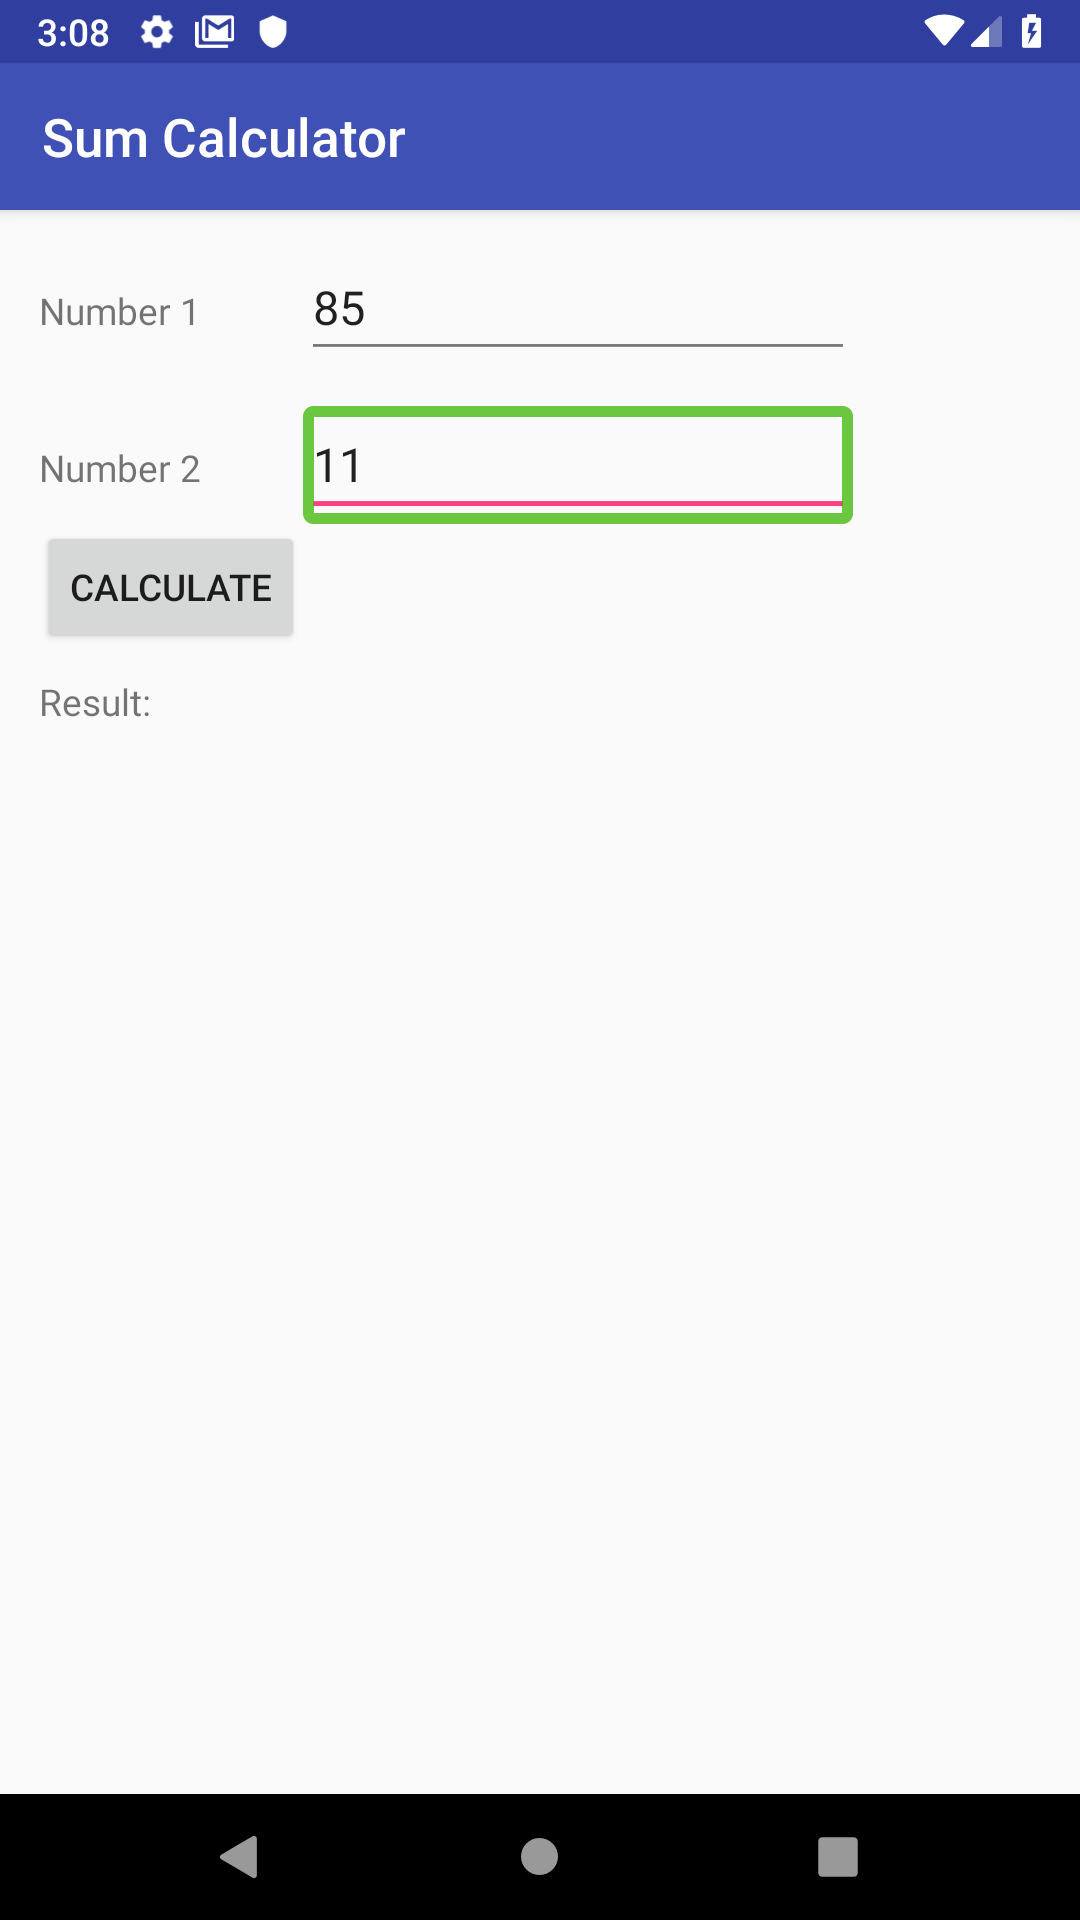
\includegraphics[width=0.4\linewidth]{img/talkback_focus}
    \caption{Groene omkadering toont focus in TalkBack }
    \label{fig:talkbackfocus}
\end{figure}

De groene omkadering in figuur \ref{fig:talkbackfocus} toont waar een gebruiker zich op focust. Alle tekst en beschrijvingen die dit element bevat zullen uitgesproken worden door TalkBack.

Wanneer er tekst gedefinieerd staat in een element bv: een knop, dan zal deze tekst steeds voorgelezen worden bij het focussen. Toch is het van groot belang dat er wanneer een element niet duidelijk genoeg is, een extra beschrijving meegegeven wordt. Dit kan bijvoorbeeld zijn wanneer men de volgende situaties heeft: 
\begin{itemize}
    \item Meerdere elementen met dezelfde naam
     \item Afbeeldingen
       \item Aanpasbare elementen (tekstvelden, ...)
\end{itemize}
Deze extra beschrijving is een 'Content Description', deze wordt samen met het elementtype steeds voorgelezen door TalkBack. 
De declaratie ervan kan statisch gebeuren bij het aanmaken van de layout. Dit kan ook op een dynamische wijze aangepast worden.



\lstinputlisting[language=XML,label=talkbackStatic, caption={Voorbeeld in XML: Declaratie van een knop, met een statische 'Content Description'},frame=single, basicstyle=\scriptsize, firstline=9,lastline=23]{../code/Android/TalkBack/app/src/main/res/layout/activity_main.xml }

\lstinputlisting[language=Java,label=talkbackDynamic, caption={Voorbeeld in Java: Indrukken van een knop resulteert in dynamisch veranderen 'Content Description'.},frame=single, basicstyle=\scriptsize, firstline=29,lastline=38]{../code/Android/TalkBack/app/src/main/java/be/pietervandendriessche/talkback/MainActivity.java}

In zowel voorbeeld \ref{talkbackStatic}, als \ref{talkbackDynamic} wordt een beschrijving gegeven aan een element. In \ref{talkbackStatic} staat deze beschrijving statisch ingesteld. Vanaf dat de desbetreffende layout op het scherm komt krijgt deze een beschrijving. Bij het voorbeeld \ref{talkbackDynamic} wordt met de code: \emph{element.setContentDescription()}, de beschrijving toegepast/verandert wanneer op het element geklikt wordt. Een combinatie van statische en dynamische toekenning van beschrijvingen is uiteraard toegelaten, en zelfs aan te raden.

Wanneer men elementen heeft die elkaar kunnen aanvullen, kan men ervoor kiezen om deze in 1 keer uit te laten spreken door TalkBack. Dit kan men bereiken door deze elementen te groeperen in een container element. Blinde gebruikers kunnen dankzij deze groepering in één keer alle nodige informatie, die ook logisch opgebouwd is, voorgelezen krijgen.
\lstinputlisting[language=XML,label=talkbackGrouping, caption={Voorbeeld in XML: Groeperen twee tekstelementen door Linearlayout},frame=single, basicstyle=\scriptsize, firstline=25,lastline=44]{../code/Android/TalkBack/app/src/main/res/layout/activity_main.xml }
In de declaratie van de layout in voorbeeld \ref{talkbackGrouping} wordt gebruik gemaakt van een `LinearLayout`-container voor de groepering van elementen. Doordat we het attribuut \emph{android:focusable="true"} toevoegen aan de container, weet TalkBack dat hij deze kan voorlezen. Voor normale gebruikers te verhinderen dat er op de container geklikt kan worden, kan het attribuut \emph{android:focusableInTouchMode="false"}  toegevoegd worden.
\begin{figure}[h!]
    \centering
    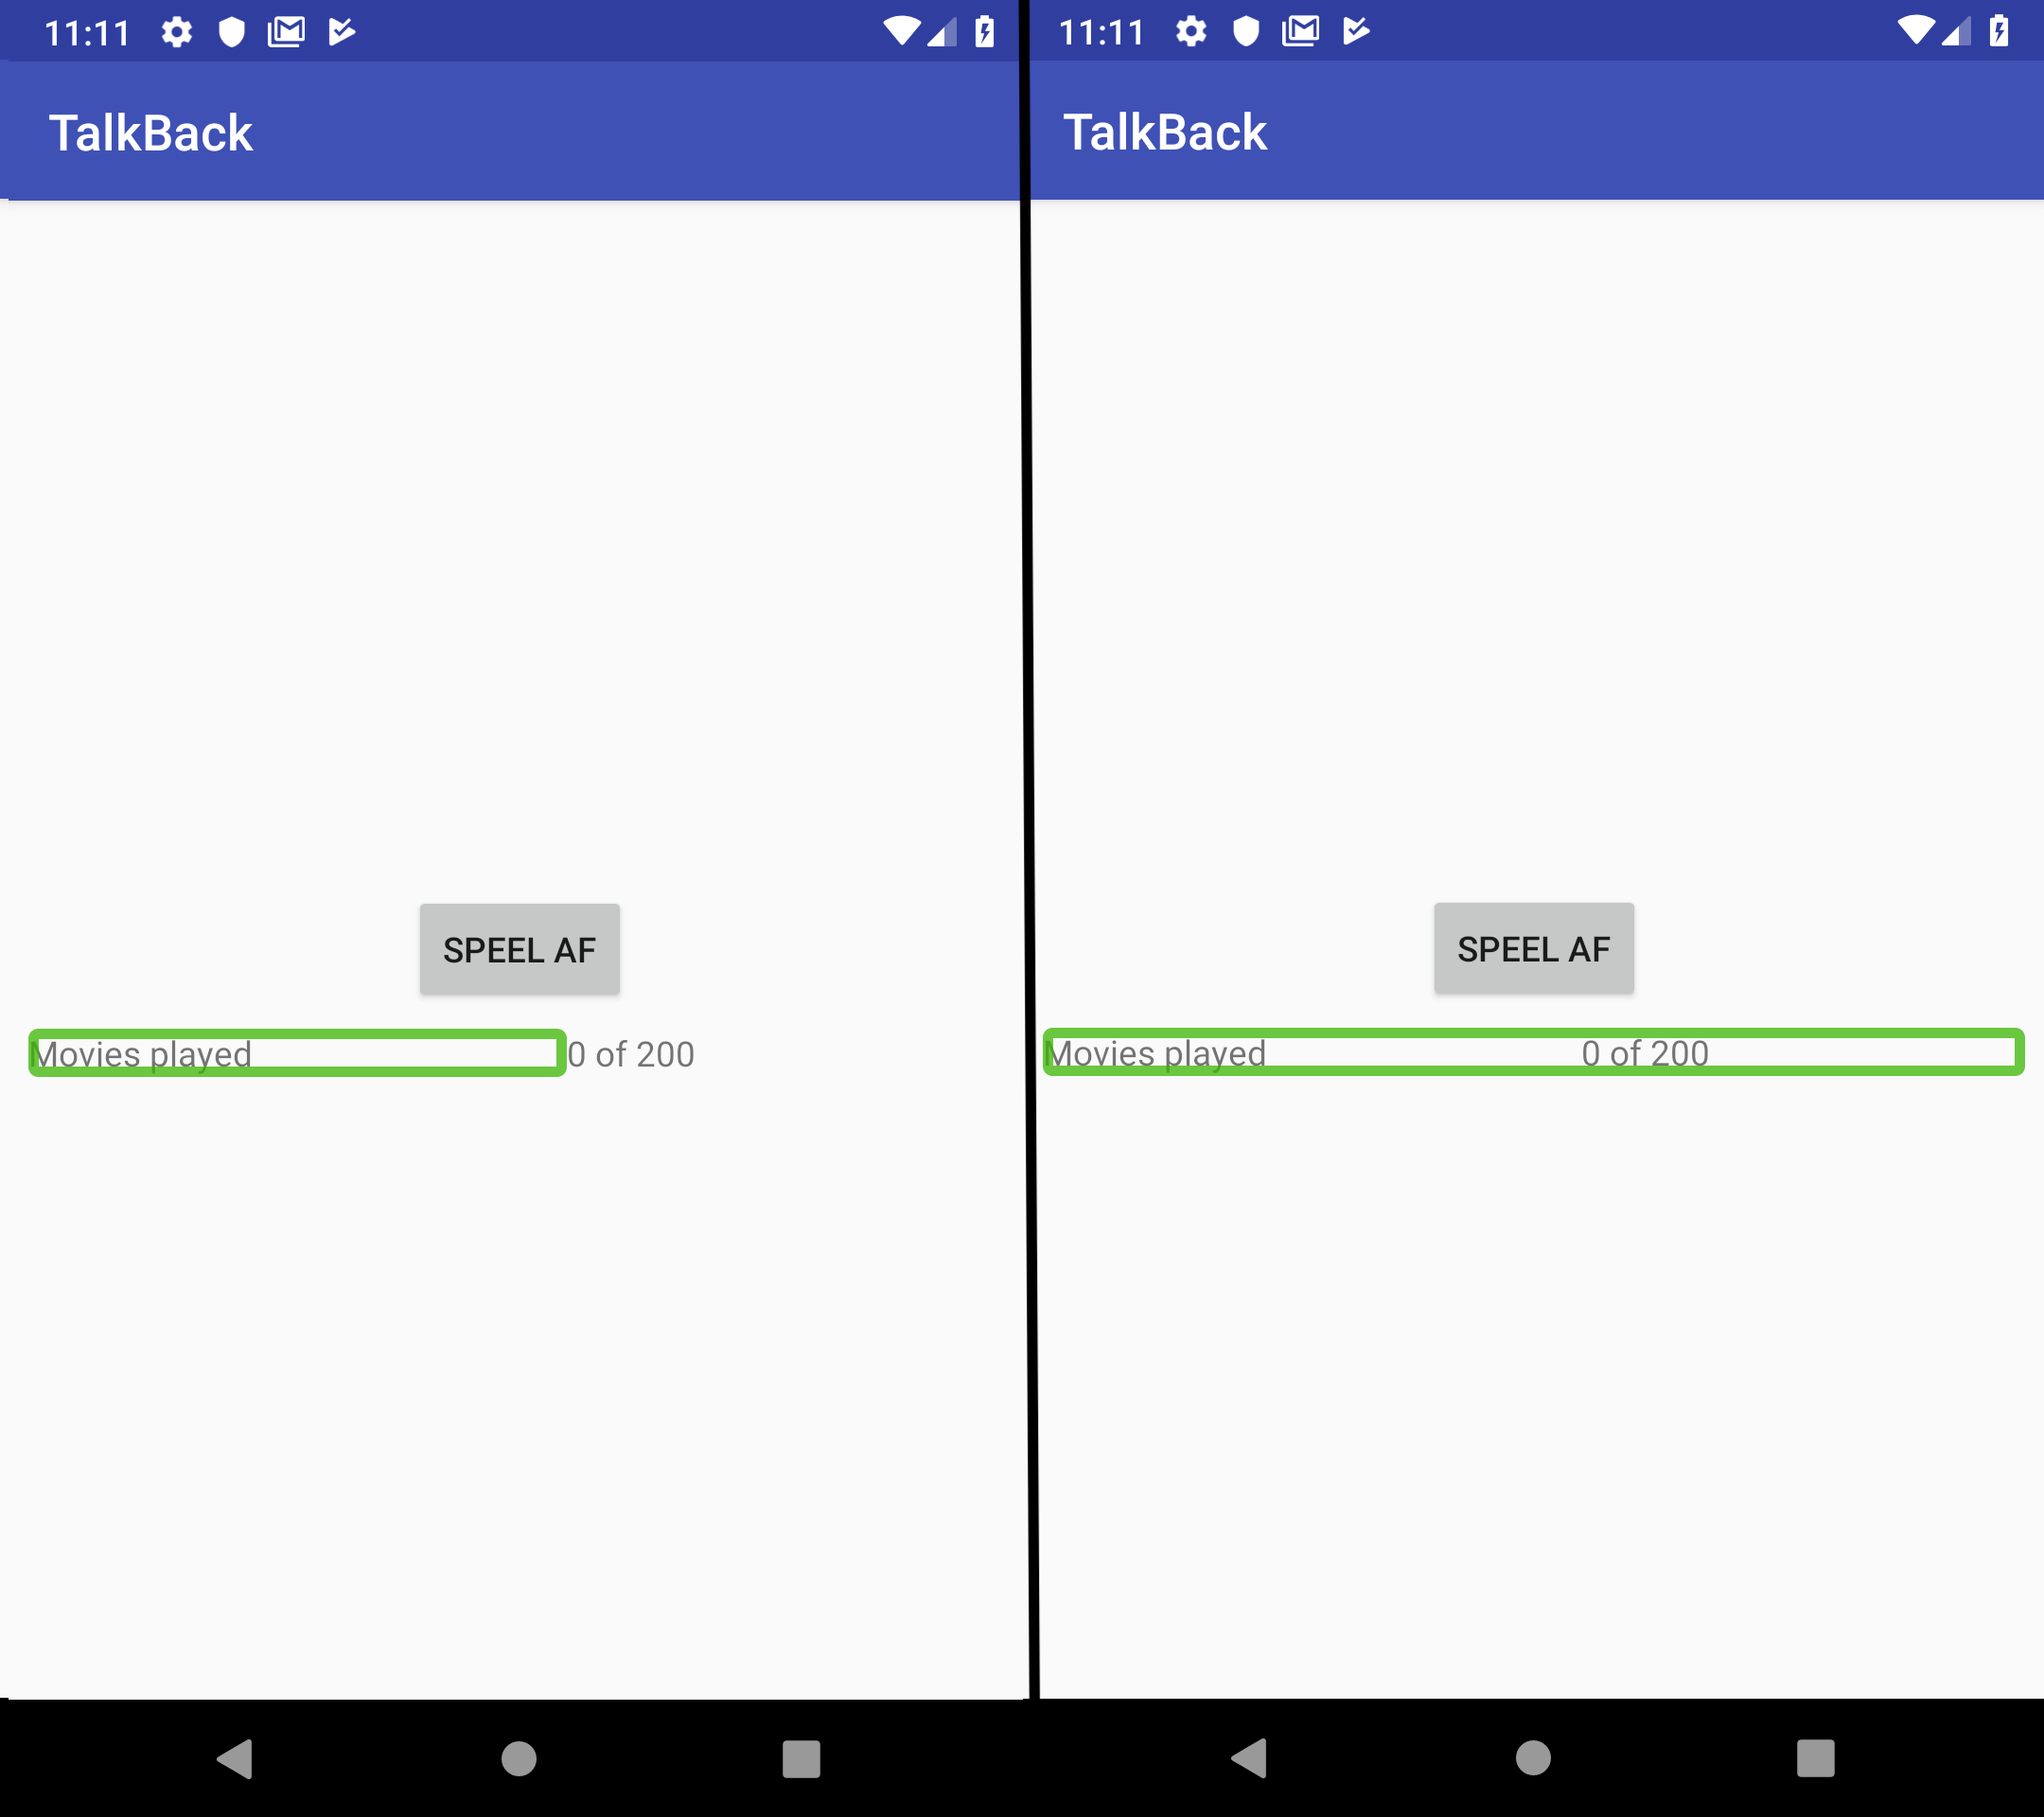
\includegraphics[width=0.6\linewidth]{img/talkback_grouped_vs_notgrouped}
    \caption{Voorbeeld van niet gegroepeerde elementen versus gegroepeerde elementen}
    \label{fig:talkbackgroupedvsnotgrouped}
\end{figure}

In figuur \ref{fig:talkbackgroupedvsnotgrouped} wordt een onderscheid gemaakt tussen een layout waar 2 gerelateerde elementen NIET gegroepeerd zijn, en een layout waarbij deze wel gegroepeerd zijn. De focus bij gegroepeerde elementen is groter, en beide elementen zullen tezamen uitgesproken worden. 

Naast het definiëren van een 'Content Description', kunnen elementen ook aankondigingen maken. Dit kan gebeuren wanneer er bijvoorbeeld een gebruiker klikt op een element, en er updaten andere elementen door die actie.
\lstinputlisting[language=Java,label=talkBackAnnounce, caption={Voorbeeld in Java: Indrukken van een knop resulteert in aankondiging TalkBack.},frame=single, basicstyle=\scriptsize, firstline=40,lastline=49]{../code/Android/TalkBack/app/src/main/java/be/pietervandendriessche/talkback/MainActivity.java}
In de code van voorbeeld \ref{talkBackAnnounce} doet de knop een aankondiging wanneer op hem geklikt wordt. De regel met code: \emph{element.announceForAccessibility()}, laat ons toe om deze aankondigingen te doen naar de eindgebruiker.

Een ontwikkelaar kan dankzij de Accessibility service API van android nagaan of TalkBack geactiveerd is. Hierdoor kunnen ze eventueel programmatisch enkele aanpassingen uitvoeren aan hun applicatie.
\lstinputlisting[language=Java,label=talkBackIsEnanled, caption={Voorbeeld in Java: Ophalen van status TalkBack},frame=single, basicstyle=\scriptsize,breaklines, firstline=23,lastline=25]{../code/Android/TalkBack/app/src/main/java/be/pietervandendriessche/talkback/MainActivity.java}

In voorbeeld \ref{talkBackIsEnanled} wordt aan de Accessibility service \gls{API} gevraagd of TalkBack geactiveerd is. De methode \emph{am.isTouchExplorationEnabled()} retourneert een boolean die overeenkomt met de activatie status van TalkBack.


\subsubsection{Vergroten lettertype}
Het aanpassen van de grote van letters kan de leesbaarheid drastisch verhogen. In Android kan de grootte van de letters aangepast worden.
Er kan gekozen worden voor de volgende groottes:
\begin{itemize}
    \item Klein
    \item Standaard
    \item Groot
    \item Grootst
\end{itemize}

Ontwikkelaars hebben de optie om de tekstgrootte in hun applicatie te definiëren aan de hand van verschillende eenheden\footnote{https://developer.android.com/guide/topics/resources/more-resources.html\#Dimension}.

Wanneer men wilt dat tekst schaalt naar gelang de gewenste tekstgrootte van de gebruiker moet men de eenheid \emph{sp (Scale-independent Pixels)} gebruiken. Deze eenheid heeft dezelfde capaciteiten als \emph{dp (Density-independent Pixels)}, maar wordt ook nog geschaald naar de eisen van de gebruiker.
\begin{figure}[h!]
    \centering
    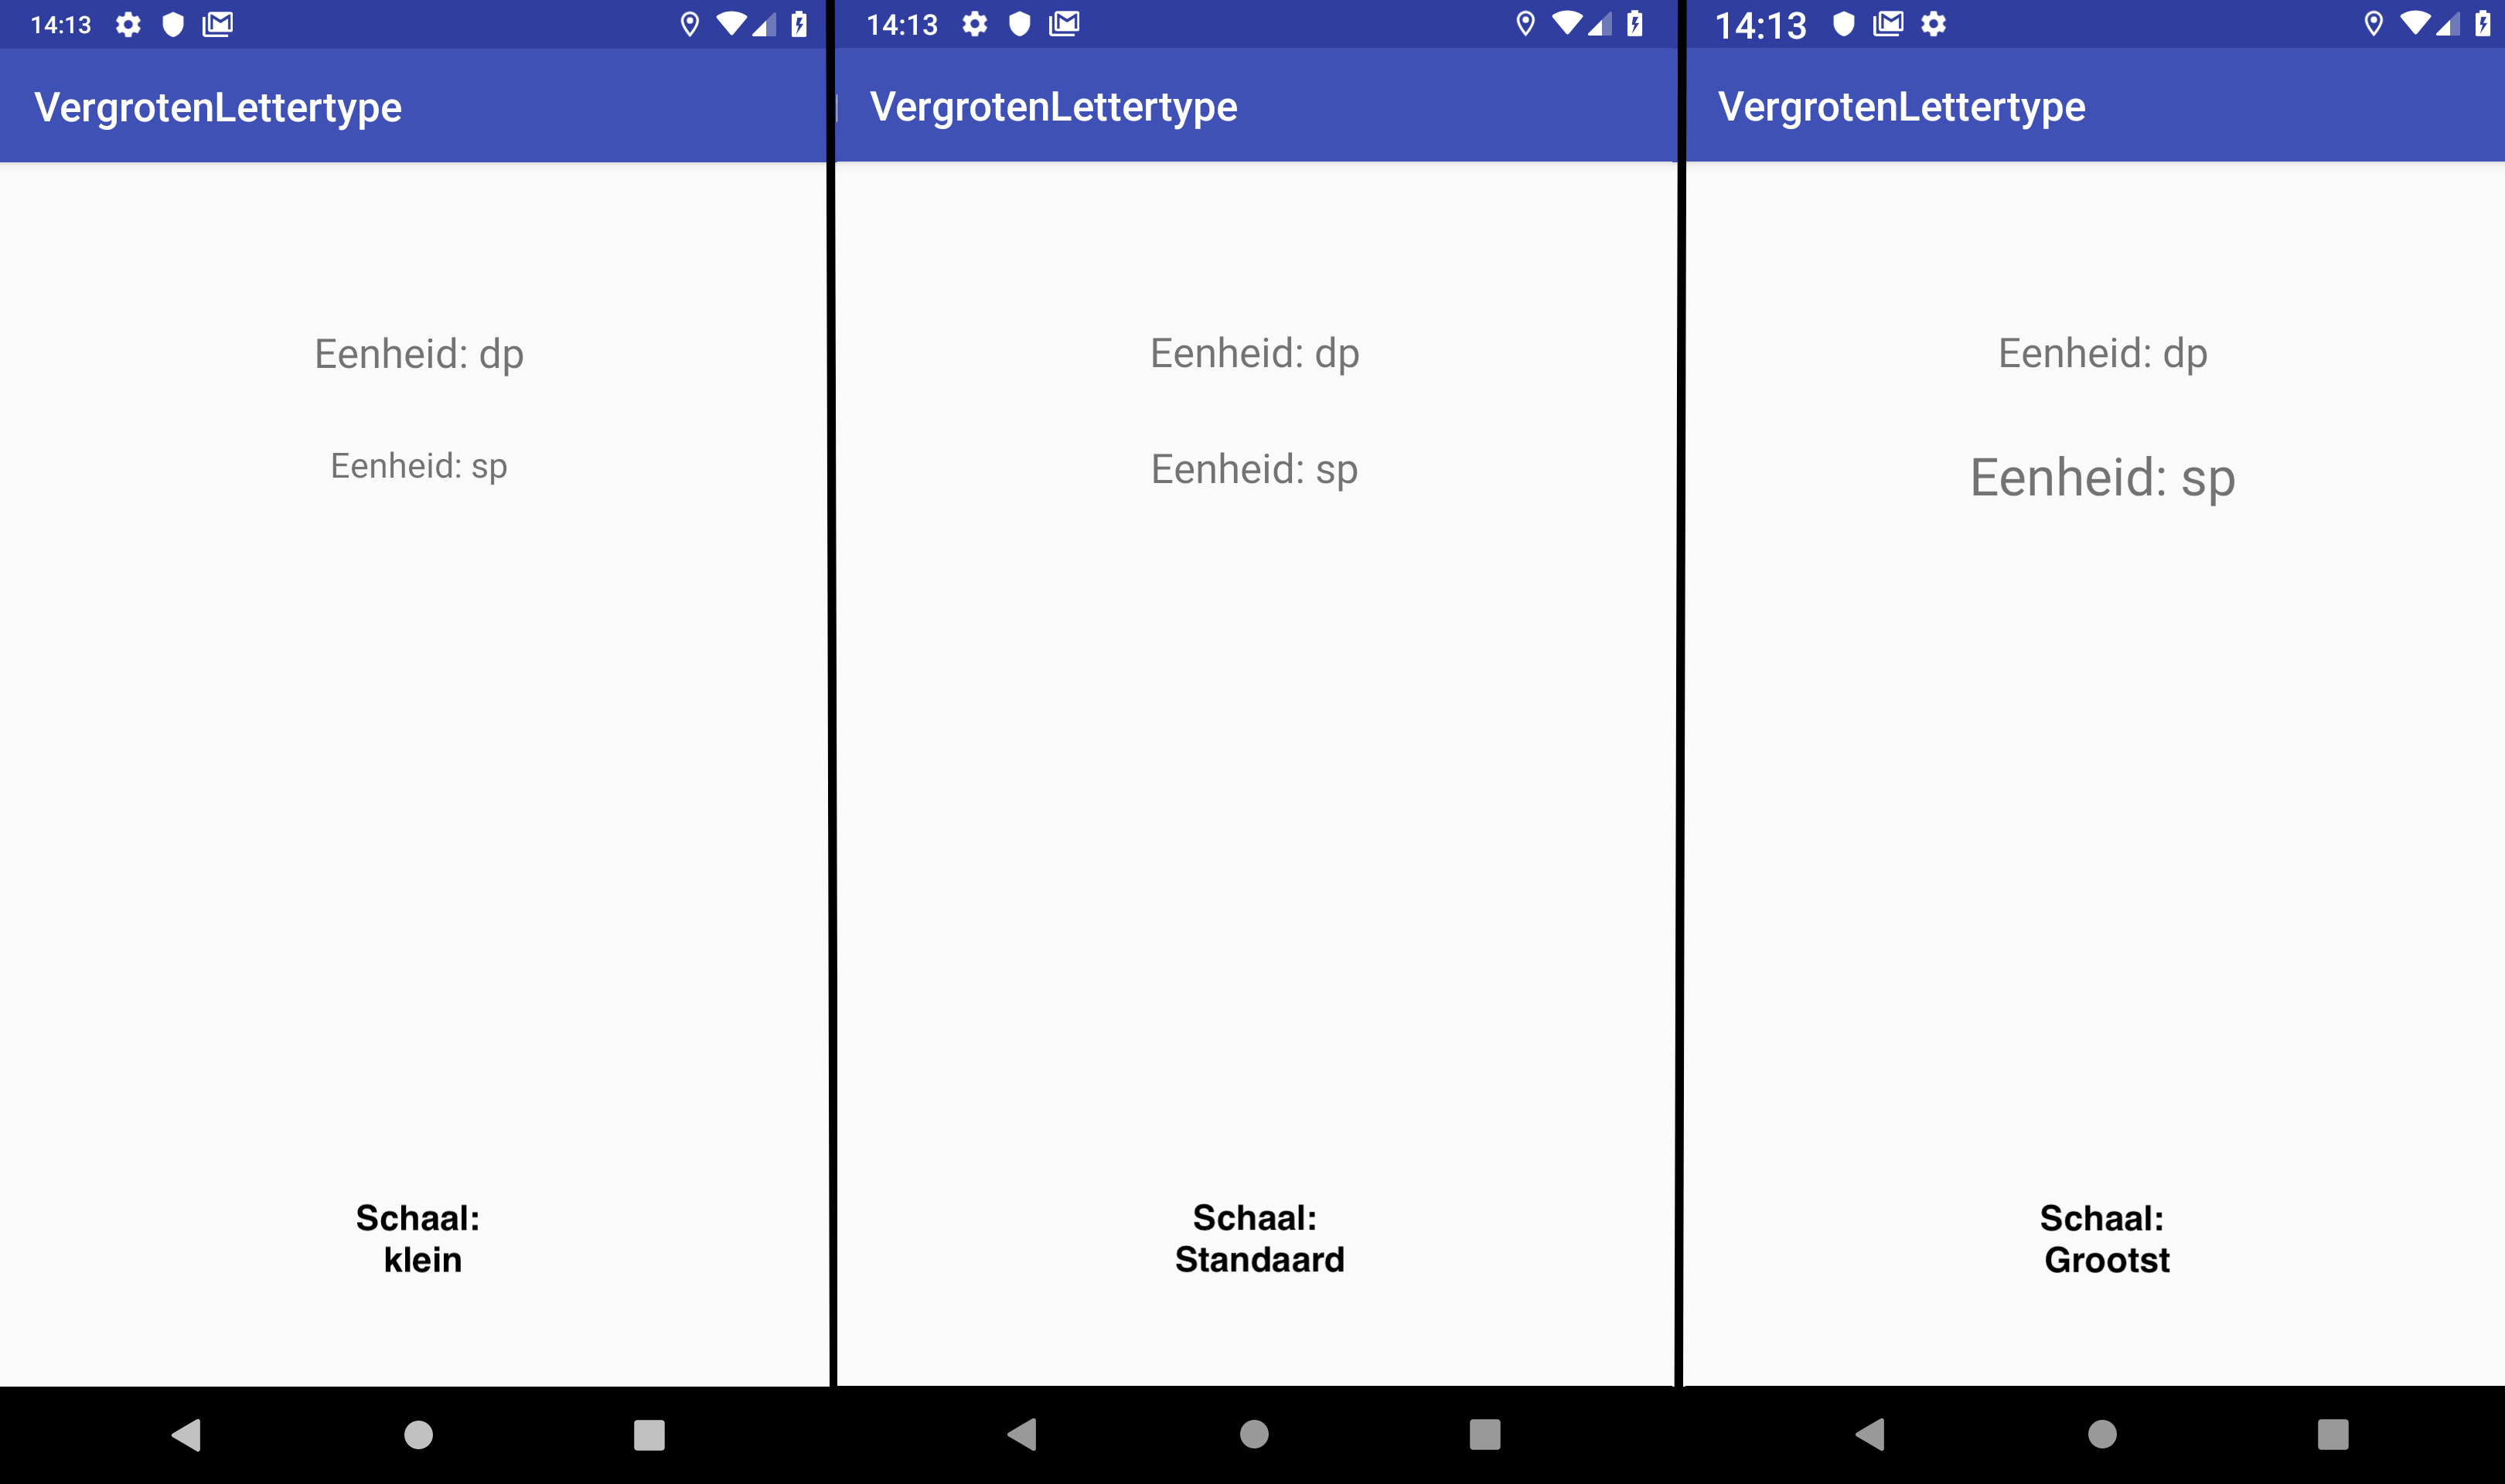
\includegraphics[width=0.8\linewidth]{img/Android_Scale_font}
    \caption{Verschil sp en dp met aanpassingen font}
    \label{fig:androidscalefont}
\end{figure}

In figuur \ref{fig:androidscalefont} is het verschil tussen sp en dp zichtbaar, in alle gevallen waar de schaal is aangepast verandert de tekst met eenheid dp niet. De tekst elementen die een grootte toegewezen hebben gekregen met de eenheid sp veranderen wel mee.



Als ontwikkelaar kan men ook nagaan welke schaal een gebruiker heeft ingesteld. Dit kan door het opvragen van de waarde van de instelling: \emph{FONT\_SCALE}.


\lstinputlisting[language=Java,label=fontscaleAndroid, caption={Voorbeeld in Java: Ophalen van schaalgrootte tekst.},frame=single, breaklines,basicstyle=\scriptsize, firstline=17,lastline=25]{../code/Android/VergrotenLettertype/app/src/main/java/be/pietervandendriessche/vergrotenlettertype/MainActivity.java }

In voorbeeld \ref{fontscaleAndroid} is er een methode die de tekstschaal ophaalt die de gebruiker heeft ingesteld.
De waarden die men zal terugkrijgen zijn respectievelijk:
\begin{itemize}
    \item Klein: 0.85
    \item Standaard: 1.00
    \item Groot: 1.15
    \item Grootst: 1.30
\end{itemize}


\subsubsection{Weergavegrootte aanpassen }
Deze functie laat een gebruiker toe om alles groter weer te geven. De elementen in een applicatie krijgen een grotere schaal. Alle elementen worden geschaald, onafhankelijk van welke eenheid men voor grootte heeft gebruikt. Dus tekst met de eenheid dp worden ook vergroot.

\subsubsection{Vergroting}
Android bevat een vergrotingsfunctionaliteit, deze zal de gebruiker toelaten om in te zoomen op het volledige scherm. Deze kan bestuurt worden met touchgebaren. 

Een ontwikkelaar kan aan individuele elementen van zijn applicatie ook een vergrotingsfunctionaliteit koppelen. Daarbij kan een gebruiker het element indrukken, en een vergroting komt tevoorschijn. 
\lstinputlisting[language=Java,label=magnifierAndroidElement, caption={Voorbeeld in Java: Toekennen van een vergrootglas aan een element},frame=single, breaklines,basicstyle=\scriptsize, firstline=20,lastline=36]{../code/Android/magnifier/app/src/main/java/be/pietervandendriessche/magnifier/MainActivity.java}
In voorbeeld \ref{magnifierAndroidElement} wordt gebruik gemaakt van de Magnifier-\gls{API} om een vergrotingsmogelijkheden te koppelen aan een element. De methode \emph{magnifier.show()} activeert het vergrootglas. De methode \emph{magnifier.dismiss()} verbergt het vergrootglas terug. In figuur \ref{fig:magnifyinapp} is er een visuele representatie van bovenstaande code.
\begin{figure}[h!]
    \centering
    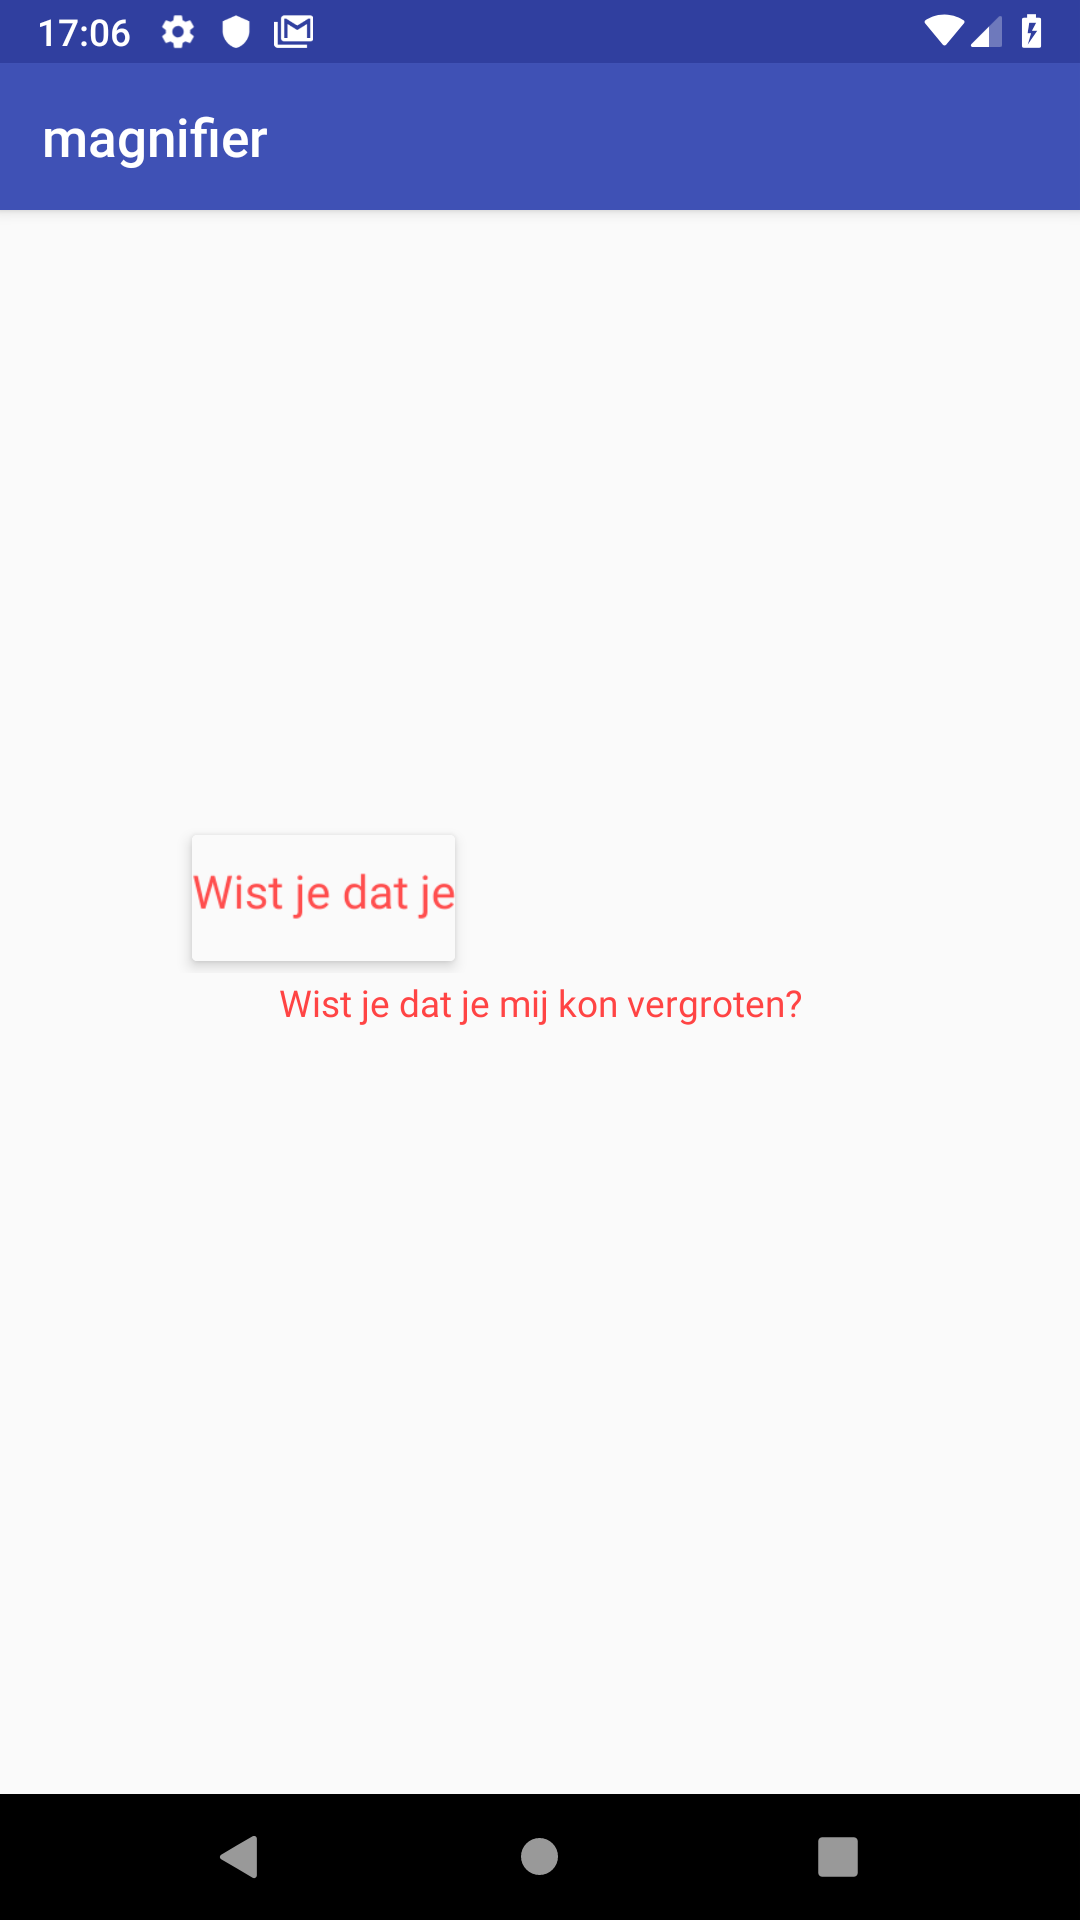
\includegraphics[width=0.4\linewidth]{img/magnify_in_App}
    \caption{Vergroten van een tekstelement}
    \label{fig:magnifyinapp}
\end{figure}
\newpage
\subsubsection{Filters voor kleurenblindheid}
Android biedt een schermfilter aan waarbij  kleuren aangepast worden zodat deze beter zichtbaar worden voor kleurenblinden. Deze filtering gebeurt dan voor alles wat op het scherm tevoorschijn komt. Sectie \ref{sec:Visueel} biedt uitleg over de verschillende soorten kleurenblindheid. Voor de 3 belangrijkste soorten kleurenblindheid worden filters voorzien. Ontwikkelaars hebben geen mogelijkheid om deze functie te faciliteren. Het gebruik van kleuren die goede contrasten hebben is wel aangeraden.



\subsubsection{Hoger contrast tekst}
Bij het gebruik van deze optie zal de kleur van tekst verdwijnen, en wordt die vervangen door zwart en wit.
In figuur \ref{fig:contrastInAndroid} is zichtbaar dat de tekst vervangen wordt voor het verhogen van het contrast. De tekst valt nu beter te onderscheiden van andere interface elementen. De functionaliteit werd geactiveerd in de rechterkant van de figuur.
\begin{figure}[h]
    \centering
    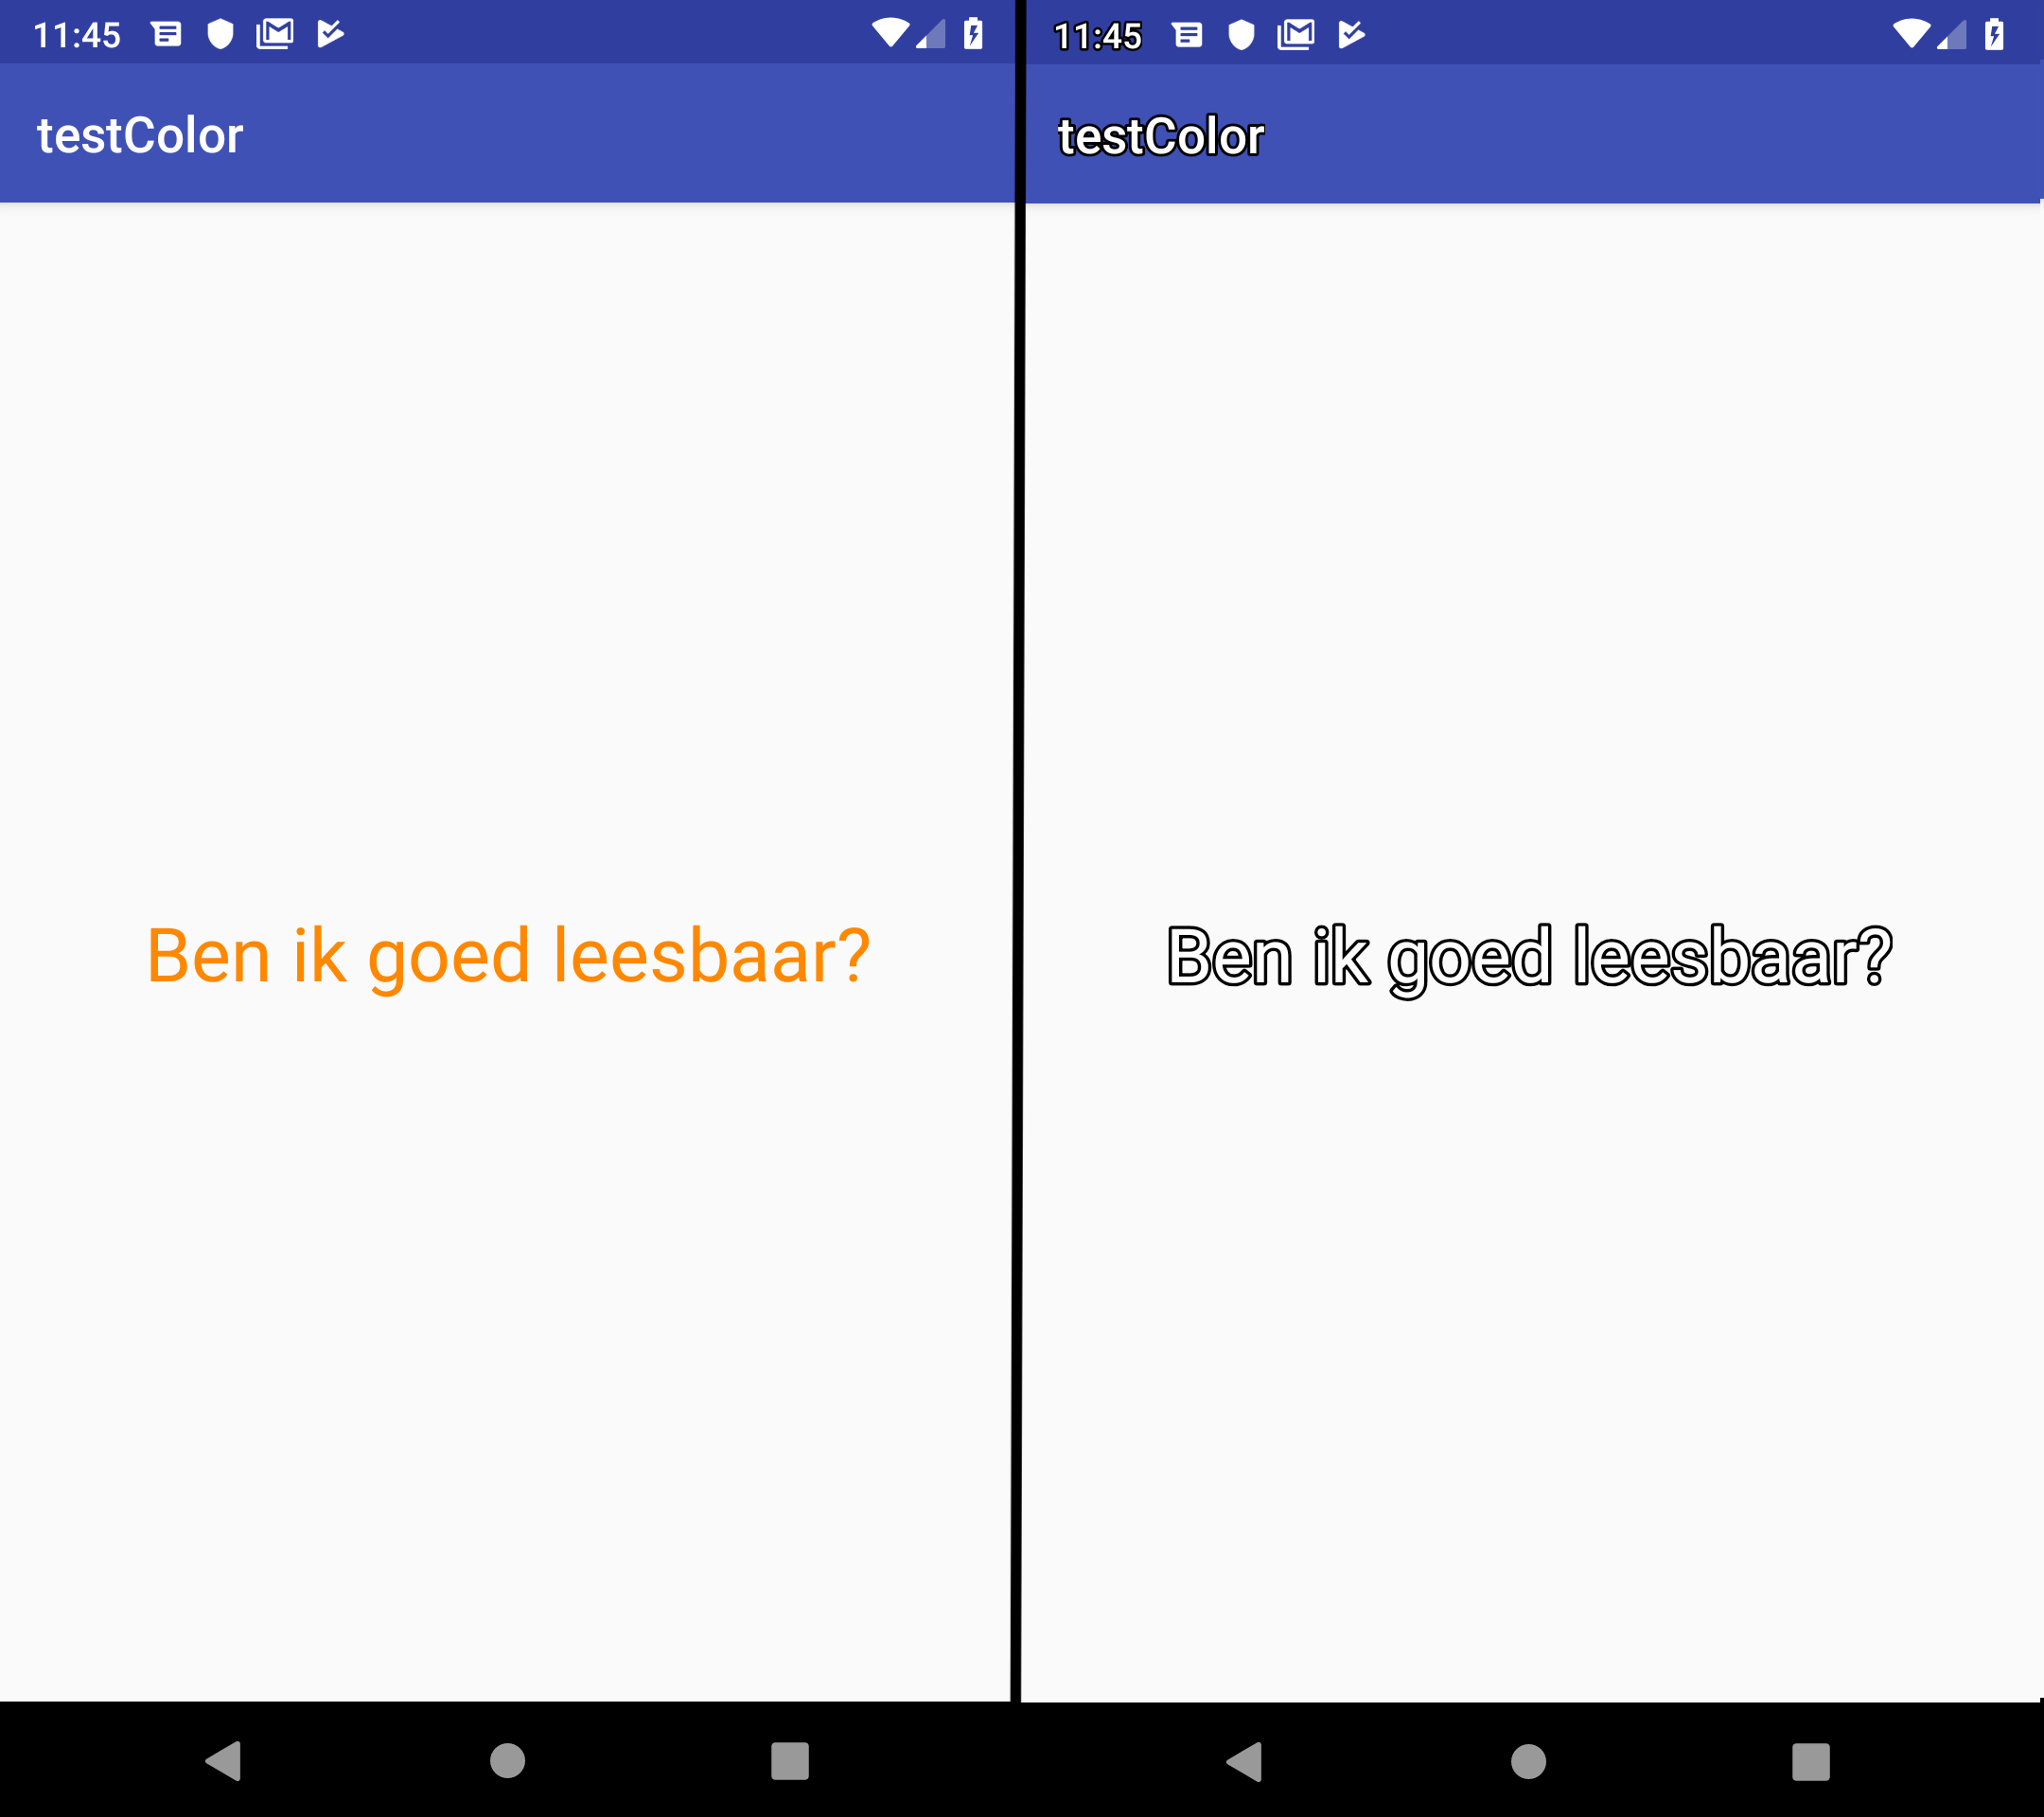
\includegraphics[width=0.6\linewidth]{img/contrastInAndroid}
    \caption{Voorbeeld hoger contrast tekst functionaliteit in Android}
    \label{fig:contrastInAndroid}
\end{figure}
\newpage
\subsubsection{Inverteren kleuren}

Het inverteren van kleuren helpt mensen met een zwak zicht om het scherm beter leesbaar te maken. Kleuren worden letterlijk geïnverteerd voor een hoger contrast te creëren. Witte achtergronden worden zwart, zwarte tekst wordt wit, etc. Deze functie fungeert als een filter en zal dus ALLE kleuren inverteren.
Naast het verhogen van de leesbaarheid voor mensen met een visuele beperking heeft deze functie ook nut voor mensen die hun smartphone in donkere ruimtes wensen te gebruiken.

\subsection{Auditief}
\subsubsection{Mono-geluid}
In sommige gevallen hebben mensen nood aan geluid vanuit 1 kant van de headset. Met deze functionaliteit wordt geluid geconverteerd naar 1 audio-kanaal in de plaats van 2. Bij stereo-geluid hoor je de audio opgesplitst in 2 audio-kanalen.

\subsubsection{Ondertitelingen}
\label{subsec:ondertitelAndroid}
Wanneer deze functionaliteit geactiveerd is kunnen mensen die doof zijn of hardhorig zijn gebruik maken van ondertitelingen in bepaalde applicaties. Android laat ook toe om voorkeuren te geven over hoe de ondertiteling getoond wordt. De voorkeuren die men kan opgeven zijn:
\begin{itemize}
\item Taal (taal waarin ondertiteling wordt weergegeven)
\item Tekengrootte (de grootte van de ondertitelingstekst)
\item Ondertitelstijl (kleur ondertitelingstekst en achtergrond)
\end{itemize}
De tekengrootte varieert van zeer klein tot zeer groot, bij de ondertitelstijl kan gekozen worden uit verschillende combinaties in letterkleur en achtergrondkleur. Een voorbeeld van hoe de ondertiteling er uit zal zien is zichtbaar wanneer men zijn voorkeuren ingeeft.

Ondertitelingen worden enkel zichtbaar wanneer deze worden toegevoegd aan een video.

\lstinputlisting[language=Java,label=AndroidAddCaptions, caption={Voorbeeld in Java: Toekennen van ondertitelingen aan een VideoView},frame=single, breaklines,basicstyle=\scriptsize, firstline=58 , lastline=60]{../code/Android/Subtitles/app/src/main/java/be/pietervandendriessche/subtitles/MainActivity.java}
In voorbeeld \ref{AndroidAddCaptions} worden ondertitelingen toegevoegd aan een VideoView. VideoView is in staat om de ondertitelingen aan te passen aan de voorkeuren van de gebruiker. Dit wil zeggen dat de ontwikkelaar geen moeite moet doen om zijn ondertitelingen aan te passen aan de voorkeuren van de gebruiker van zijn applicatie.
\lstinputlisting[language=Java,label=AndroidCaptionsInformation, caption={Voorbeeld in Java: Toekennen van ondertitelingen aan een VideoView},frame=single, breaklines,basicstyle=\scriptsize, firstline=24,lastline=28]{../code/Android/Subtitles/app/src/main/java/be/pietervandendriessche/subtitles/MainActivity.java}
Wanneer een ontwikkelaar niet gebruik maakt van een VideoView, maar wel van ondertitelingen moet men de waarden van de voorkeuren van de gebruiker opvragen. Aan de hand van die waarden kan de ontwikkelaar de ondertiteling aanpassen aan de voorkeuren. In voorbeeld \ref{AndroidCaptionsInformation} wordt via de \emph{CaptionManager} nagegaan welke voorkeuren een gebruiker heeft. Elk type voorkeur heeft een corresponderende methode.

\lstinputlisting[language=Java,label=AndroidCaptionsInformationEventHandler, caption={Voorbeeld in Java: Eventhandler bij het veranderen van voorkeuren ondertitelingen},frame=single, breaklines,basicstyle=\scriptsize, firstline=32,lastline=53]{../code/Android/Subtitles/app/src/main/java/be/pietervandendriessche/subtitles/MainActivity.java}

Men kan ook een Eventhandler koppelen aan de \emph{CaptionManager}, wanneer een voorkeur veranderd of de ondertiteling wordt uitgeschakeld kan dat opgevangen worden. Voorbeeld \ref{AndroidCaptionsInformationEventHandler} toont hoe deze Eventhandler gedefinieerd kan worden en hoe welke veranderingen in voorkeuren men kan opvangen. Bij elke methode die zo'n verandering opvangt krijgt men de nieuwe waarde mee wanneer een verandering is gebeurd.
\subsubsection{Geluidsversterker}
De geluidsversterker functionaliteit in Android laat een gebruiker toe om geluiden in sterkte aan te passen. Een gebruiker kan zwakkere geluiden luider laten klinken, maar ook de verhinderende geluiden stiller maken. Wanneer men een koptelefoon gebruikt kan het geluid per oor geregeld worden.
\subsection{Motorisch}
\subsubsection{Toegang via schakelaars}
Gebruikers met een motorische beperking kunnen aan de hand van een schakelaar (extern apparaat) de smartphone bedienen. Alle elementen op het scherm worden overlopen, wanneer het element dat men wenst aangeduid is moet men een bepaalde toets indrukken. Via het systeem van het scannen van de elementen, en het indrukken van toetsten kan er genavigeerd worden \autocite{switchAndroid}.

Er zijn verschillende soorten schakelaars die gebruikt kunnen worden: 
\begin{itemize}
    \item Externe schakelaar
    \item Extern toetsenbord
    \item Fysieke knoppen smartphone
\end{itemize}

    \lstinputlisting[language=Java,label=switchAccessAndroid, caption={Voorbeeld in XML: ImageView klikbaar in Toegang via schakelaars},frame=single, breaklines,basicstyle=\scriptsize, firstline=9,lastline=20]{../code/Android/SwitchAccess/app/src/main/res/layout/activity_main.xml}

Wanneer een bepaald element niet gescant wordt binnen een applicatie moet men dat element 'klikbaar' maken. Met het XML-attribuut \emph{android:clickable=''true''} maakt men een element 'klikbaar'. In voorbeeld \ref{switchAccessAndroid} werd een ImageView 'klikbaar' gemaakt door het toevoegen van het XML-attribuut.
\\
Ontwikkelaars kunnen deze functionaliteit testen door een extern toetsenbord toe te voegen of gebruik te maken van de fysieke knoppen. Meer informatie over hoe men dit kan testen kan gevonden worden in de developer guide 'Test your app's accessibility' .\footnote{https://developer.android.com/guide/topics/ui/accessibility/testing}
\subsubsection{Scherm automatisch draaien}
Gebruikers met een fysieke beperking kunnen vaak moeite ervaren met het draaien van hun scherm. Daardoor is het voor hun wenselijk dat hun scherm in dezelfde rotatie blijft gedurende het gebruik. De functie 'scherm automatisch draaien' laat een gebruiker toe om in te stellen of het scherm automatisch draait.

Ook de gebruiker zonder beperking heeft voordeel bij deze functie. Men kan het automatisch roteren blokkeren wanneer dit gewenst is.

\subsubsection{Vertraging voor blijvend aanraken}
In Android kunnen gebruikers bij het klikken op een element vaak nog extra opties of acties krijgen. Dit komt doordat men dat element 'blijvend aanraakt'. Standaard moet men heel kort blijven indrukken om deze extra opties of acties te krijgen. 

Bij sommige gebruikers, waaronder vooral mensen met een motorische beperking zorgt deze korte periode dat er ongewenst acties uitgevoerd worden. Android heeft een functionaliteit waarbij men kan instellen hoelang het systeem moet wachten tot hij het registreert als een 'blijvende aanraking', gebruikers kunnen kiezen uit:
\begin{itemize}
    \item Kort
    \item Medium
    \item Lang
\end{itemize}
In bepaalde smartphones die Android draaien kan men zelfs het aantal seconden ingeven voordat het systeem het moet detecteren als een 'blijvende aanraking'. 
\subsubsection{Hardware shortcut voor activatie functionaliteiten}
De volumeknop van een Android smartphone kan gebruikt worden voor het activeren van een toegankelijkheidsfunctionaliteit. Dit laat mensen met een beperking toe om gemakkelijk hun meest gebruikte functionaliteit in te schakelen. Dankzij deze functionaliteit wordt de navigatie naar de instellingen voor de ingestelde functionaliteit overbodig.
\subsection{Cognitief}
 
\subsubsection{Animaties verwijderen}
Animaties kunnen mensen met een cognitieve beperking afleiden, frustreren of verwarren. Daarom bezit Android een functionaliteit die deze animaties compleet van het mobiele platform doet verdwijnen. Alle afleidende animaties vinden niet meer plaats.

\section{Toegankelijkheidsfunctionaliteiten in iOS}
\label{sec:ToegankelijkheidsfunctionaliteiteniOS}
\subsection{Visueel}

\subsubsection{VoiceOver}
\label{subsec:VoiceOver}
VoiceOver laat een iOS gebruiker navigeren aan de hand van audio feedback. VoiceOver zal wanneer deze geactiveerd is alle elementen op het scherm voorlezen. Men kan zonder te kijken navigeren in iOS enkel op geluid en met gebruik van je vingers. VoiceOver kent verschillende gebaren die men kan gebruiken om te navigeren als ook een rotor. Deze rotor laat je efficiënt navigeren binnen de applicatie, hij past zich aan eraan. VoiceOver bevat tal van functionaliteiten die zeer wenselijk zijn, zo kan je bij het gebruik van een koptelefoon een audiokanaal kiezen voor de audio feedback. Een persoon met een beperking kan zijn ervaring met VoiceOver volledig personaliseren.

\begin{figure}[h]
    \centering
   \frame{ 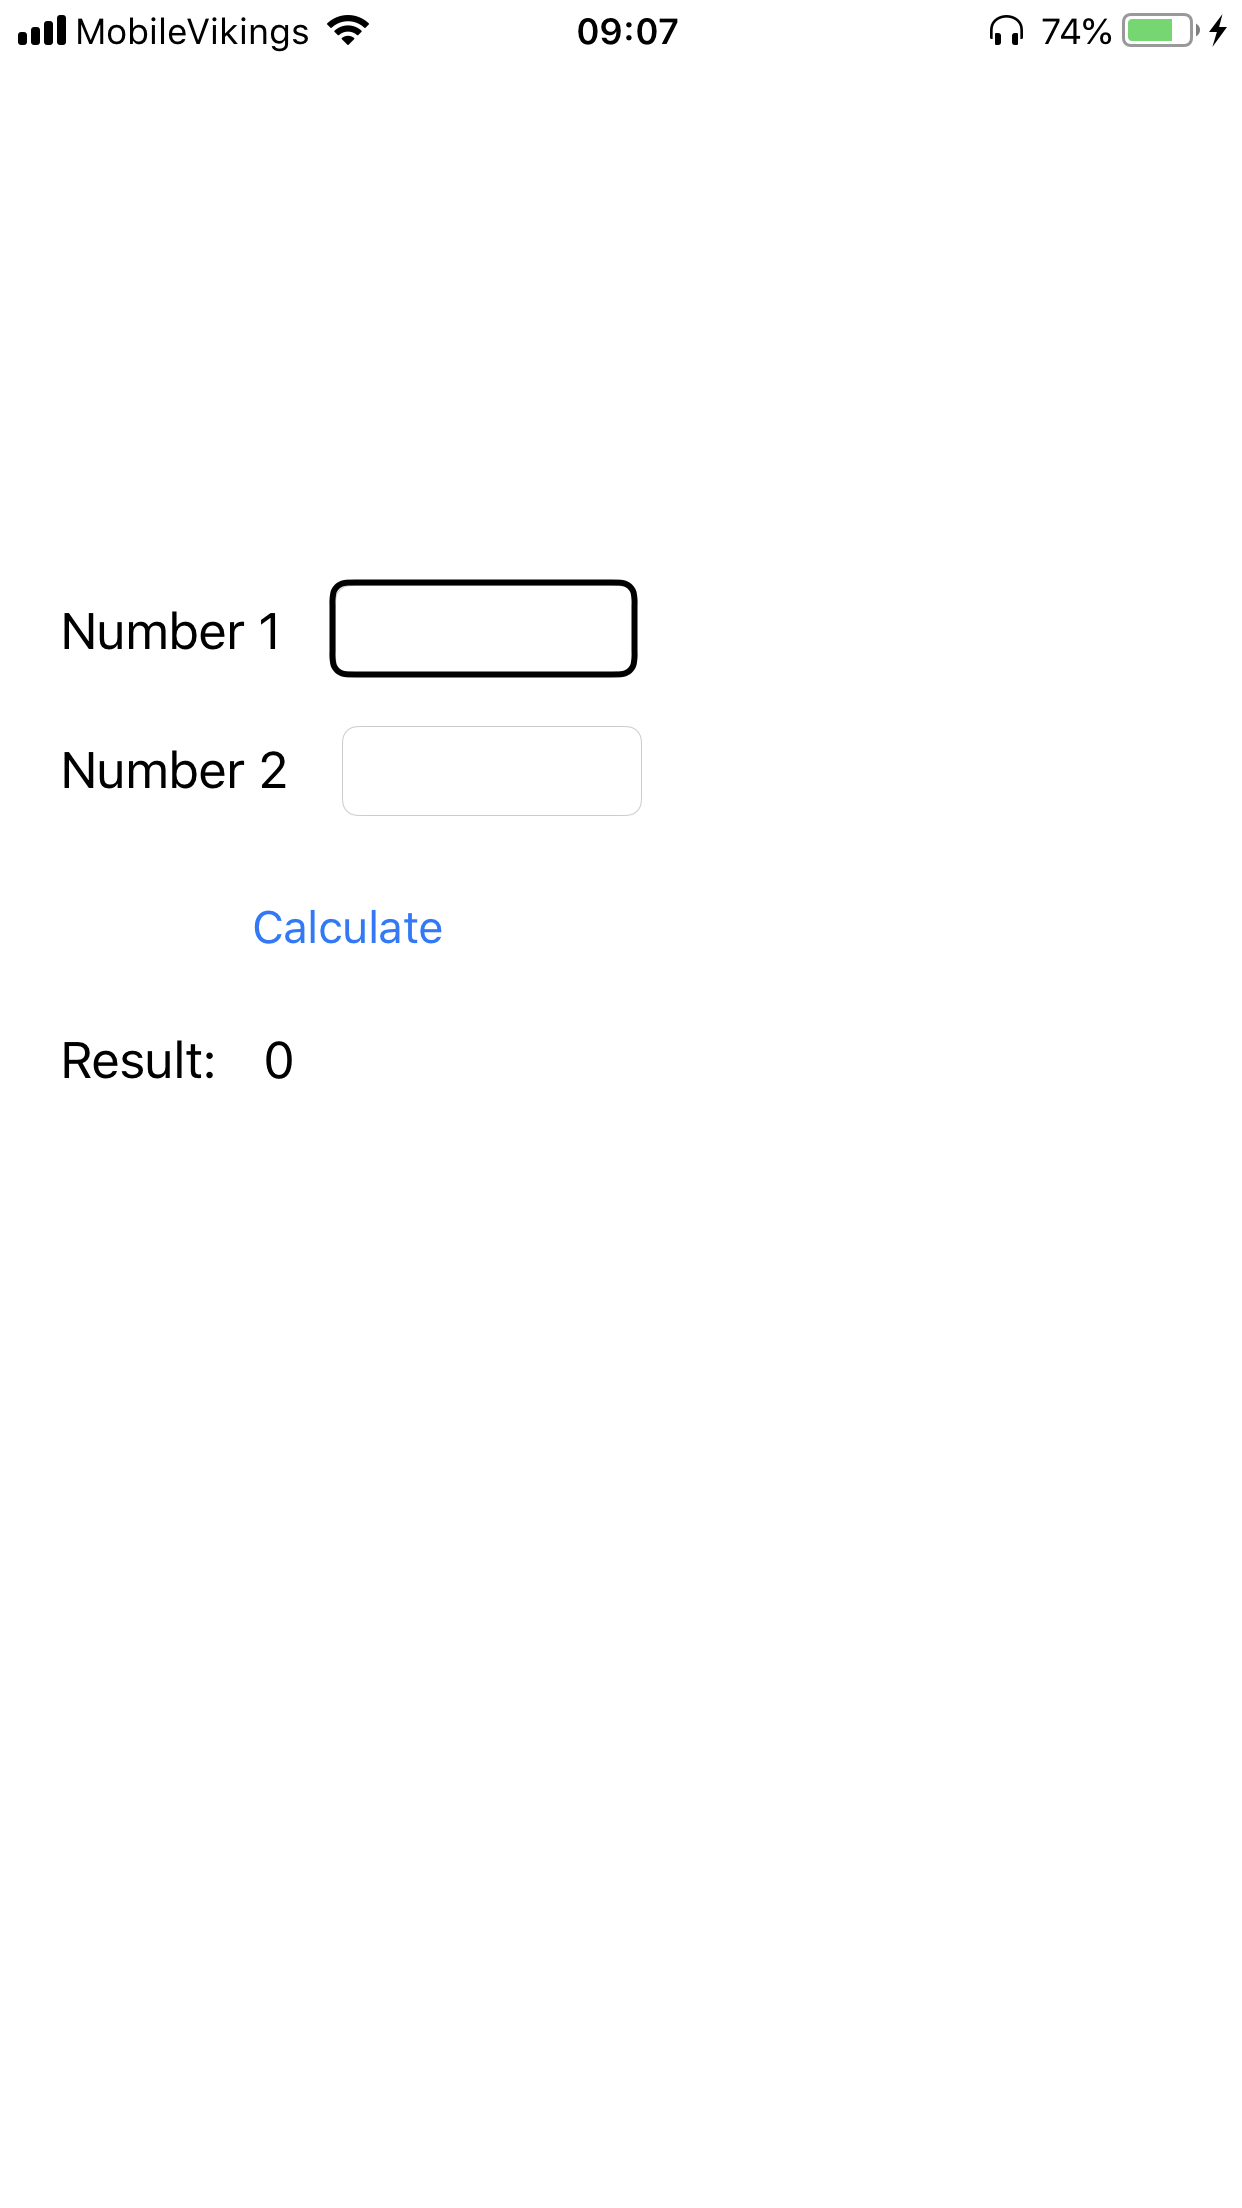
\includegraphics[width=0.35\linewidth]{img/VoiceOver_focus}}
    \caption{Zwarte omkadering toont focus in VoiceOver }
    \label{fig:VoiceOverfocus}
\end{figure}

In figuur \ref{fig:VoiceOverfocus} toont de zwarte omkadering waar de gebruiker op dat moment op gefocust is. Het element die de focus heeft zal uitgesproken worden door VoiceOver. In het geval van figuur \ref{fig:VoiceOverfocus} wordt ook de inhoud van het TextField uitgesproken.

Zoals in Android's TalkBack zal de tekst die gedefinieerd staat steeds uitgesproken worden. Toch is het steeds van belang om een zinvolle beschrijving te geven aan elementen. 
In VoiceOver wordt een ImageView niet standaard voorgelezen, een ontwikkelaar moet het element inschakelen voor toegankelijkheid. Dit kan dynamisch gedaan worden, maar ook bij het declareren van de elementen in het 'Storyboard'.
\newpage
In VoiceOver kunnen naast een beschrijving kunnen ook andere verschillende waarden toegevoegd worden om VoiceOver te laten uitspreken. Enkele hiervan zijn:
\begin{itemize}
    \item Label: beschrijving van het element (bijvoorbeeld: Foto van een honds)
    \item Traits: eigenschappen van het element (bijvoorbeeld: knop, geselecteerd, header, ...)
    \item Hints: Beschrijft welke actie een element kan volbrengen (bijvoorbeeld: verhogen van waarde)
\end{itemize}

    \lstinputlisting[language=java,label=dynamicAccessVoiceOverDescription, caption={Voorbeeld in Swift: Toekennen van een beschrijving aan een ImageView},frame=single, breaklines,basicstyle=\scriptsize, firstline=29,lastline=34]{../code/iOS/VoiceOver/VoiceOver/ViewController.swift}

In voorbeeld \ref{dynamicAccessVoiceOverDescription} wordt er dynamisch een beschrijving toegekend aan een ImageView. De regel met \emph{element.isAccessibilityElement = true} zorgt dat het element gevonden kan worden door VoiceOver.  Bepaalde elementen zoals een ImageView worden niet standaard gevonden door VoiceOver, deze dienen eerst geactiveerd te worden. De regel \emph{element.accessibilityLabel = "beschrijving"} laat ons toe om dynamisch een beschrijving te koppelen aan een element.

    \lstinputlisting[language=java,label=dynamicAccessVoiceOverTrait, caption={Voorbeeld in Swift: Toekennen van eigenschap knop aan ImageView},frame=single, breaklines,basicstyle=\scriptsize, firstline=36,lastline=39]{../code/iOS/VoiceOver/VoiceOver/ViewController.swift}

Voorbeeld \ref{dynamicAccessVoiceOverTrait} toont dan weer hoe men VoiceOver aangeeft dat de ImageView niet enkel een foto is, maar ook een knop. Dit gebeurt door de regel \emph{petPicture.accessibilityTraits.insert()}, waarbij we de eigenschap 'knop' toevoegen aan de ImageView.

    \lstinputlisting[language=java,label=dynamicAccessVoiceOverHint, caption={Voorbeeld in Swift: Toekennen van een hint aan een Button},frame=single, breaklines,basicstyle=\scriptsize, firstline=41,lastline=43]{../code/iOS/VoiceOver/VoiceOver/ViewController.swift}
    Wanneer men wilt vertellen wat er gebeurt wanneer men een bepaalde knop indrukt kan men best een hint toevoegen. In voorbeeld \ref{dynamicAccessVoiceOverHint} wordt gebruik gemaakt van een hint wanneer men op de knop drukt. Deze wordt uitgesproken bij het focussen op de knop. De regel \emph{element.accessibilityHint = "hintBeschrijving"} laat ons toe om een hint toe te kennen aan een element.
    
   Naast het dynamisch instellen van beschrijvingen voor het verhogen van de toegankelijkheid met VoiceOver, kan dit ook op een statische manier. Dit gebeurt wanneer men de verschillende elementen declareert in het Storyboard.
   
   Dit kan wanneer men in de  'Storyboard editor' een element selecteert en de 'identity inspector' opent. In de 'identity inspector' kan men de sectie 'accessibility' vinden. 
   \newpage
   \begin{figure}[h]
       \centering
       \frame{ 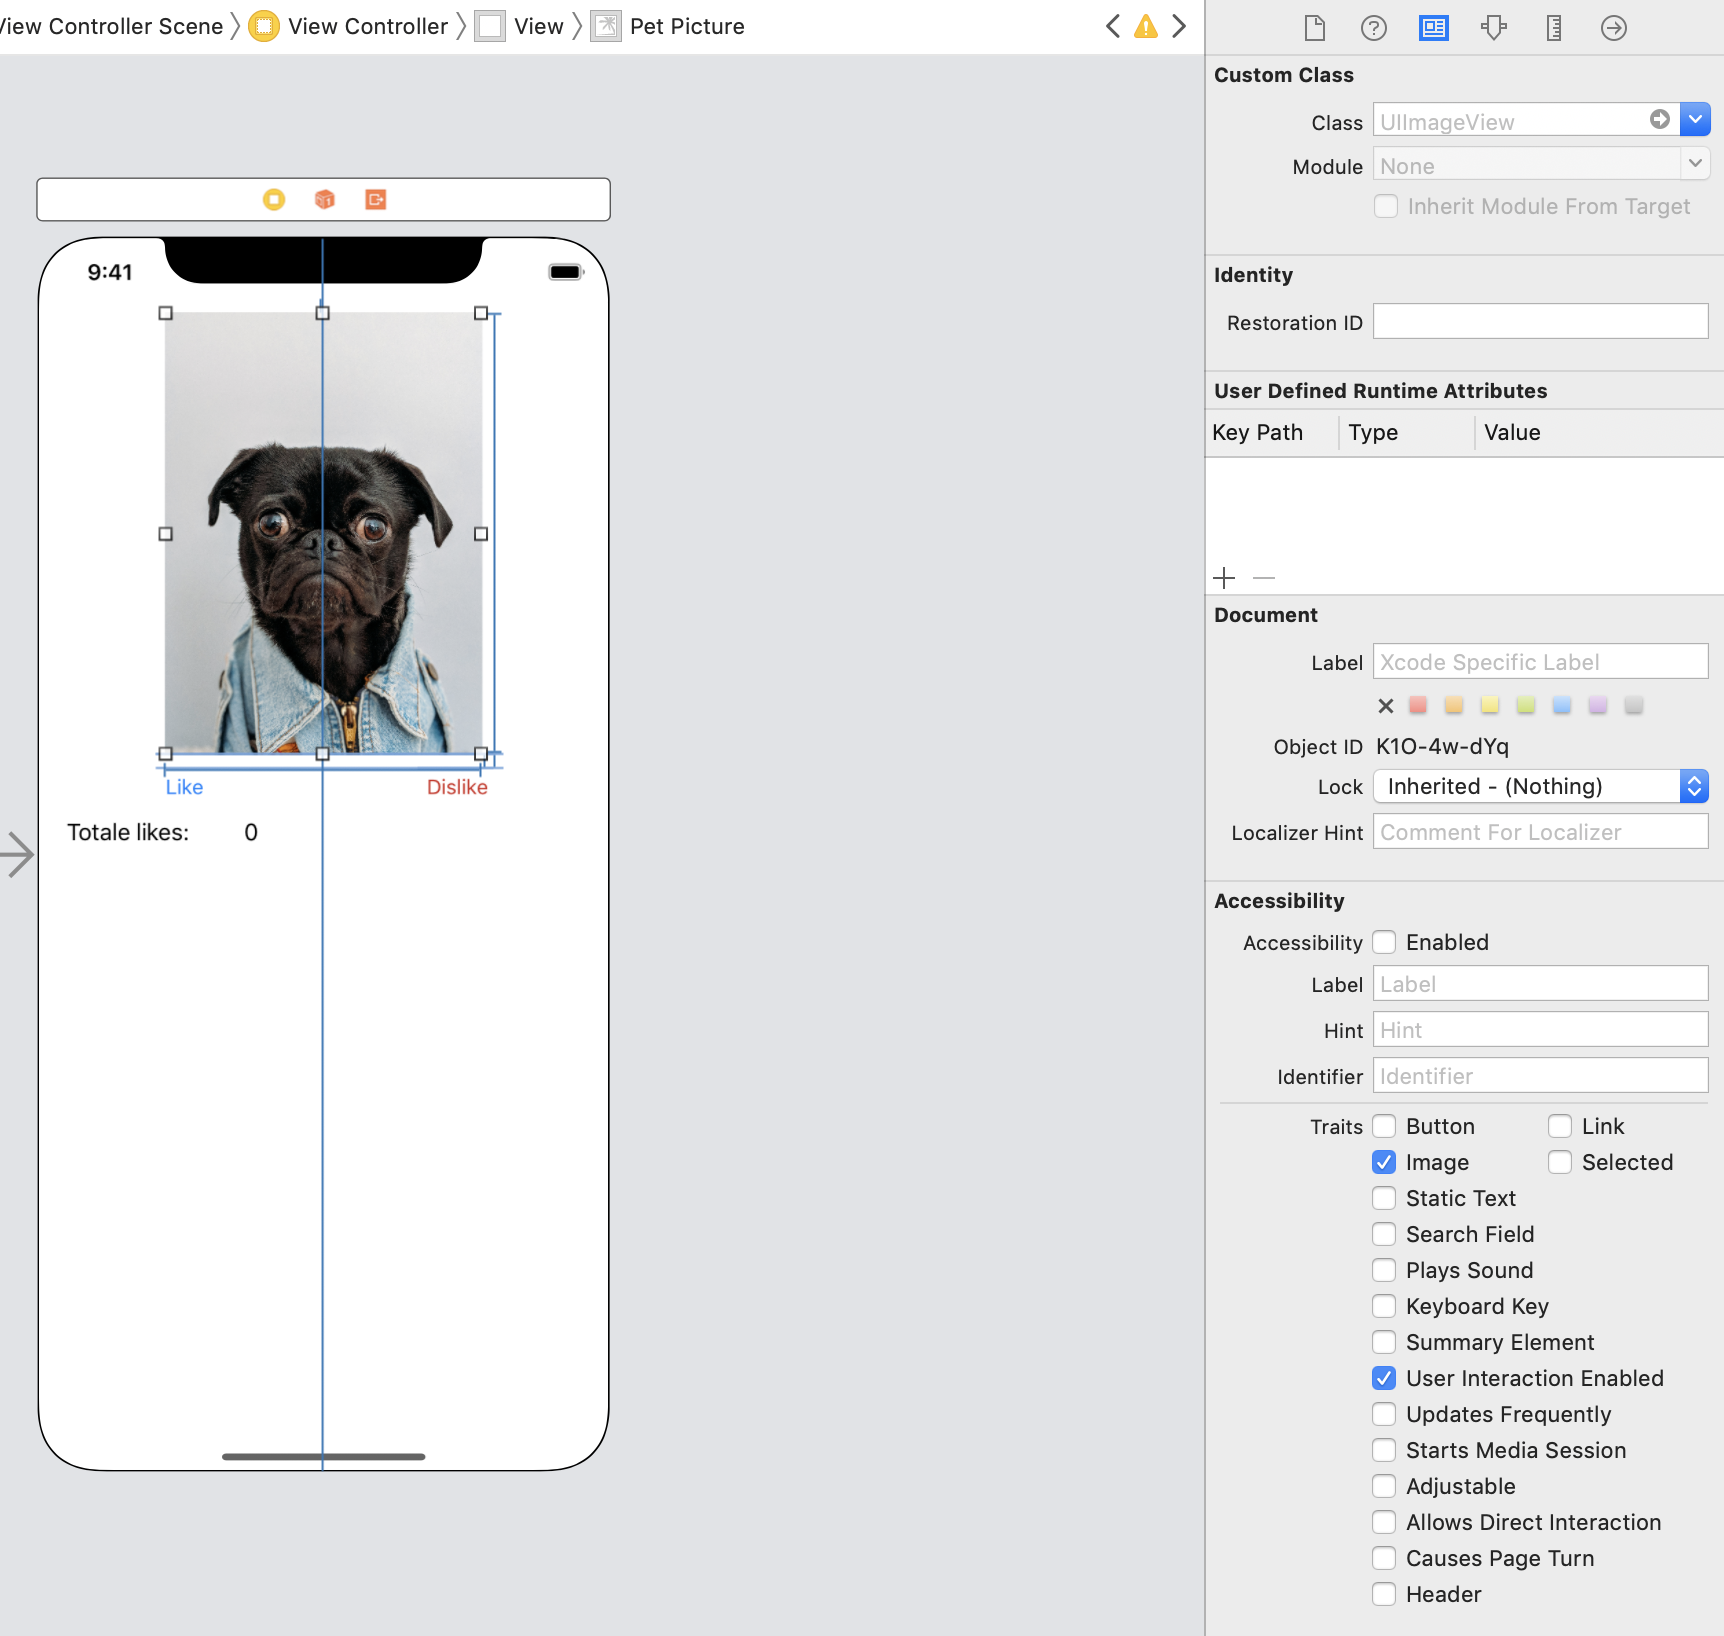
\includegraphics[width=0.7\linewidth]{img/storyboardAccessibility}}
       \caption{Voorbeeld van sectie 'accessibility' in de 'identity inspector' van een Storyboard }
       \label{fig:storyboardAccessibility}
   \end{figure}
In figuur \ref{fig:storyboardAccessibility} werd een afbeelding geselecteerd, bij deze afbeelding staat 'Accessibility' niet aangevinkt. Dit wil zeggen dat VoiceOver dit element niet zal voorlezen. Verder kan men een beschrijving toevoegen in het veld 'Label', een hint in het veld 'Hint'. Ook kunnen er eigenschappen toegevoegd worden door deze in de sectie 'Traits' aan te vinken.
 \lstinputlisting[language=java,label=dynamicAccessVoiceOverGrouping, caption={Voorbeeld in Swift: Toekennen van een beschrijving voor gegroepeerde elementen},frame=single, breaklines,basicstyle=\scriptsize, firstline=44,lastline=49]{../code/iOS/VoiceOver/VoiceOver/ViewController.swift}

Voorbeeld \ref{dynamicAccessVoiceOverGrouping} toont hoe men elementen kan groeperen en VoiceOver die ook kan laten uitspreken als een gegroepeerd element. In iOS volstaat het niet enkel om de elementen te groeperen en een attribuut aan te passen. In voorbeeld \ref{dynamicAccessVoiceOverGrouping} wordt er voor een StackView met 2 labels een beschrijving toegekend. De regel \emph{element.accessibilityElements = []} is noodzakelijk om VoiceOver duidelijk te maken welke elementen gegroepeerd zijn. Daarnaast moeten er kenbaar maken dat de groepering mag gezien worden door VoiceOver, dit gebeurt met de regel \emph{element.isAccessibilityElement = true}. Als laatste wordt er in de laatste regel een beschrijving van de container toegekend.
\newpage
   \begin{figure}[h]
    \centering
    \frame{ 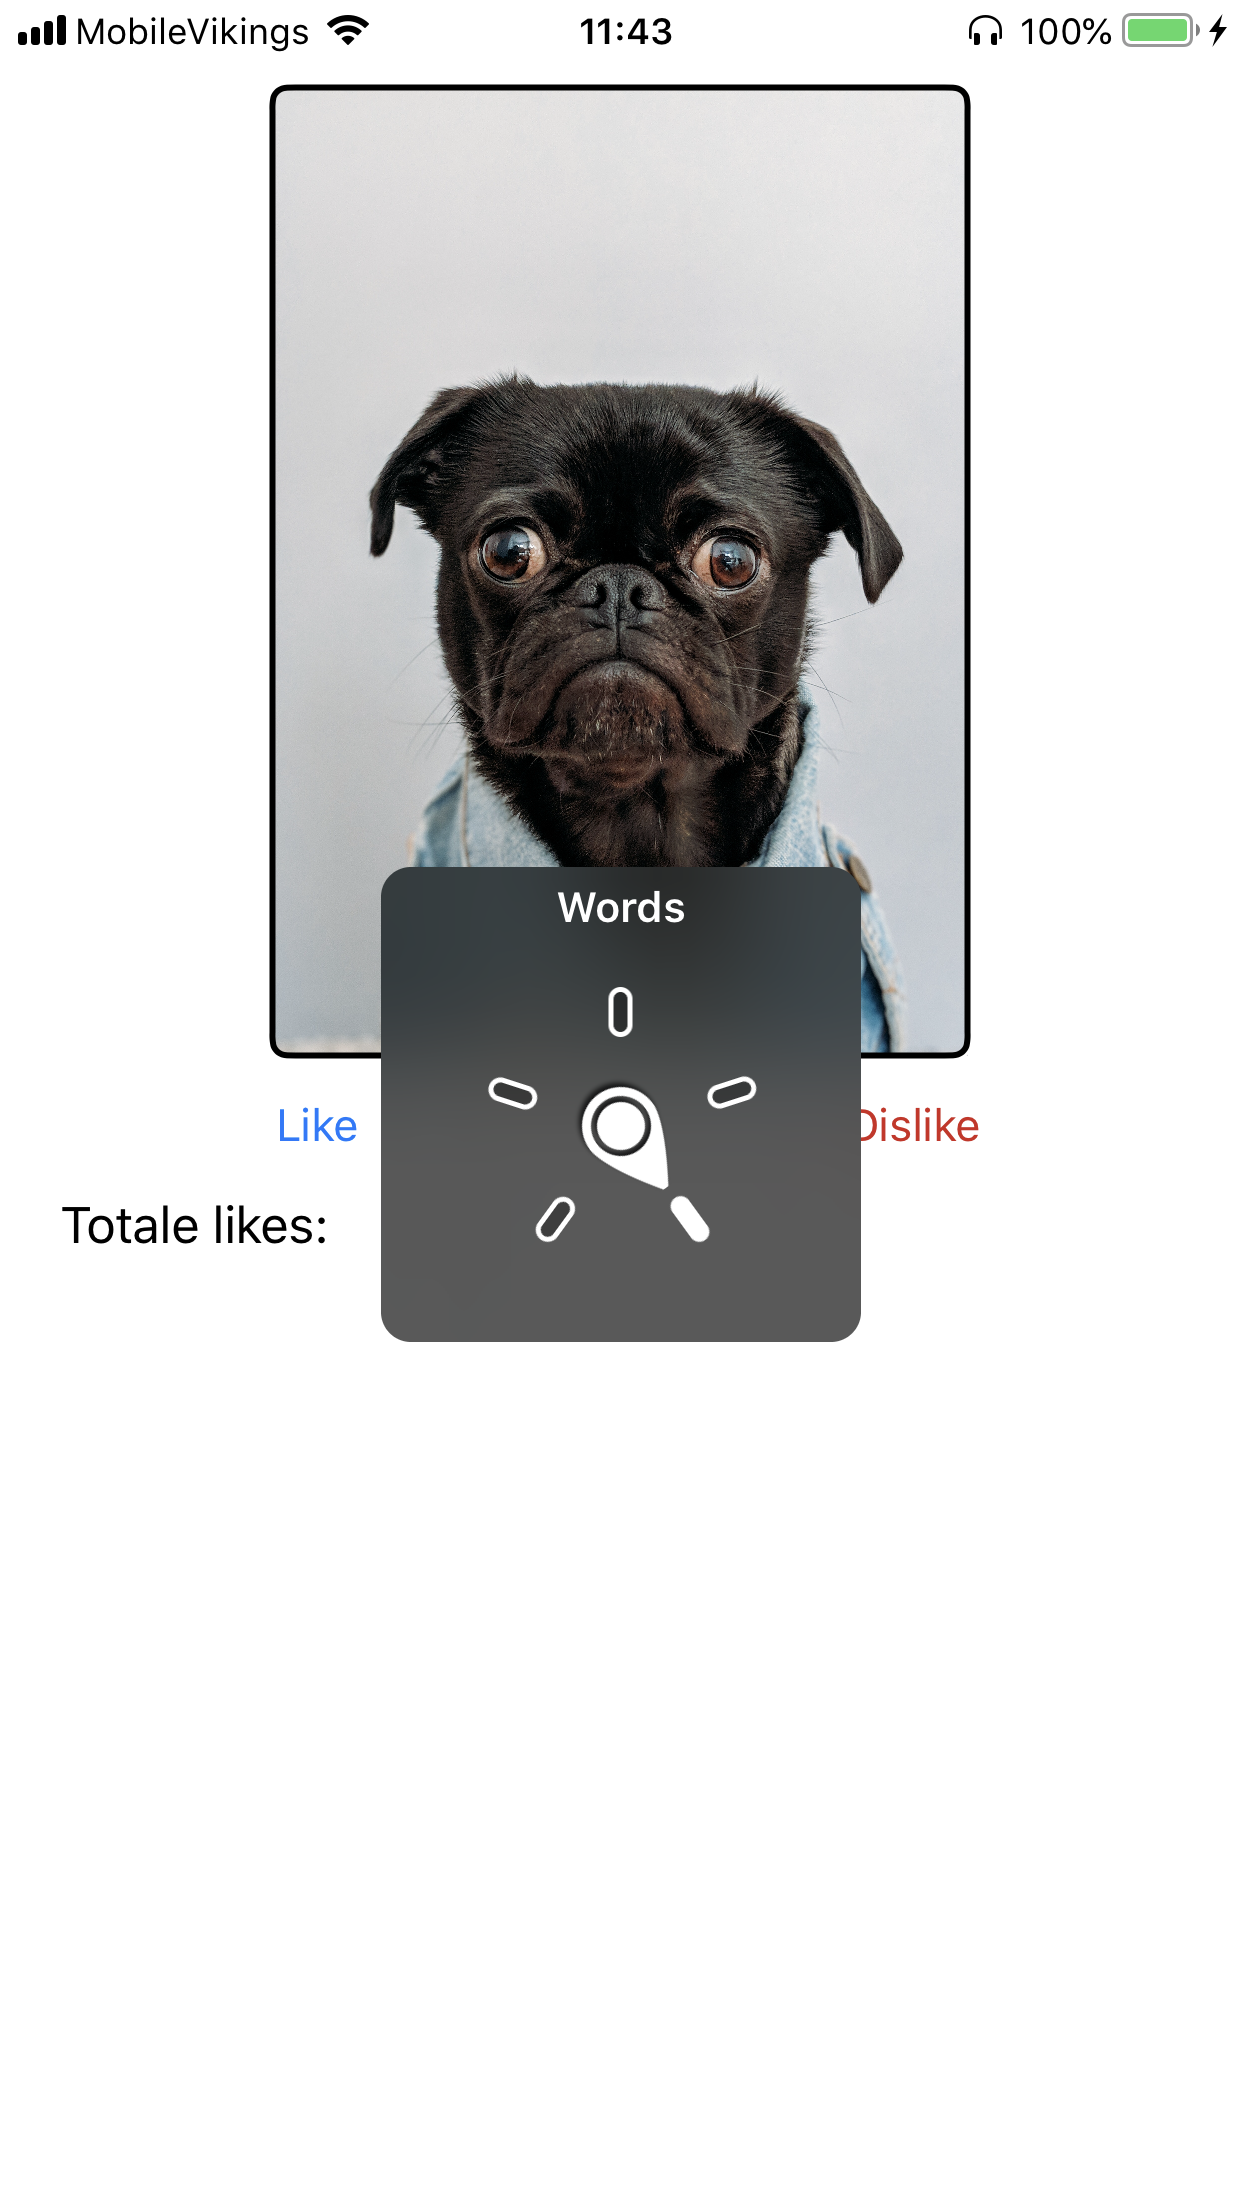
\includegraphics[width=0.3\linewidth]{img/rotor}}
    \caption{Voorbeeld van rotor in VoiceOver }
    \label{fig:voiceOverRotor}
\end{figure}
VoiceOver bevat een functionaliteit waarbij gebruikers makkelijk door verschillende soorten elementen kunnen scrollen. Deze functionaliteit heet 'rotor', en kan men gebruiken door een draaibeweging te maken met 2 vingers wanneer VoiceOver is geactiveerd. In voorbeeld \ref{fig:voiceOverRotor} wordt het scrollen tussen alle verschillende woorden geactiveerd. Men kan scrollen tussen de elementen door met je vinger omhoog of omlaag te slepen.

Als ontwikkelaar is het mogelijk om een filter toe te voegen aan de rotor voor gebruik binnen zijn applicatie.  Meer informatie daarover is te vinden in de developer documentatie van Apple\footnote{\url{https://developer.apple.com/documentation/uikit/uiaccessibilitycustomrotor}}. Een ontwikkelaar kan dankzij de property \emph{UIAccessibility.isVoiceOverRunning} nagaan of deze functionaliteit is ingeschakeld. 

\subsubsection{Zoom}
Zoom is een functie in iOS die toelaat om in te zoomen op het volledige scherm. Deze functie fungeert letterlijk als een vergrootglas in de display van je iOS smartphone. Aan de hand van enkele gebaren kan je deze functie besturen. Zo is het dubbel tappen met 3 vingers de functie activeren. Ook is deze functionaliteit is voldoende te personaliseren naar de noden van de gebruiker. Één van de mogelijkheden tot personaliseren is dat men kan kiezen uit het zoomen in een bepaald frame, of het volledige scherm te laten zoomen. Ook kan men instellen dat bij het inzoomen een filter op de zoom komt, deze filters kunnen het volgende: \begin{itemize}
    \item Kleuren inverteren
    \item Kleuren omzetten naar grijswaarden
    \item Kleuren inverteren en omzetten naar grijswaarden
    \item Kleuren verminderen en contrast verhogen voor weinig licht
\end{itemize}

\subsubsection{Vergrootglas}
De functie Vergrootglas laat een gebruiker toe om zijn camera te laten werken als een vergrootglas. De functie wordt geactiveerd door driemaal kort de homeknop in te drukken. 
Slechtzienden kunnen dankzij deze functie de wereld rondom zich vergroten. Wanneer men de functie heeft geactiveerd kan men allerlei filters activeren om de zichtbaarheid te verhogen.
\subsubsection{Inverteren kleuren}
Deze functionaliteit bevat 2 opties, namelijk 'Slim omgekeerd'  en 'Klassiek omgekeerd'. Bij 'Slim omgekeerd' worden de kleuren geïnverteerd behalve die van afbeeldingen, media en apps die voldoende donkere kleuren bevatten. 'Klassiek omgekeerd' inverteert alle kleuren die op de display komen.

Bij de optie 'Slim omgekeerd' worden enkel in vooraf geïnstalleerde applicaties de kleuren van afbeeldingen niet geïnverteerd.  Een ontwikkelaar kan voorkomen dat de kleuren van een element geïnverteerd worden door de volgende regel uit te voeren op het element: \emph{element.accessibilityIgnoresInvertColors = true}.

Een ontwikkelaar kan dankzij de property \emph{UIAccessibility.isInvertColorsEnabled} nagaan of deze functionaliteit is ingeschakeld. 
\subsubsection{Kleurenfilters}
Aan de hand van deze functionaliteit kunnen kleuren aangepast weergegeven worden, zodat deze zichtbaarder zijn voor kleurenblinden. Deze filtering gebeurt over de volledige display. Bij deze functie kan ook de intensiteit van de kleurenfilterring ingesteld worden. De volgende filters zijn voorzien in deze functionaliteit: \begin{itemize}
    \item Grijstinten
    \item Rood/groen-filter (Protanoop)
    \item Groen/rood-filter (Deuteranoop)
    \item Blauw/geel-filter (Triranoop)
        \item Kleurentint (instellen van een eigen gekozen kleur)
\end{itemize}
\subsubsection{Vergroten tekst}
iOS heeft een functionaliteit die een gebruiker toelaat om de grootte van het lettertype in te stellen. Bij deze functionaliteit heeft de gebruiker een groot aantal opties voor het vergroten van het lettertype. In applicaties wordt de grootte van het lettertype geschaald naar gelang de instelling van de gebruiker. Een ontwikkelaar moet aandacht besteden voor het ondersteunen van deze schaalbare lettertypes. In tegenstelling van Android gaat iOS niet standaard alle lettertypen schalen.
In iOS wordt er een onderscheid gemaakt tussen 3 verschillende soorten lettertypes:
\begin{itemize}
    \item System
    \item Text styles
    \item Custom
\end{itemize}
Enkel de soort 'Text styles' zal automatisch schalen naar de voorkeur van de gebruiker. Wanneer men gebruikt maakt van de soort 'Custom' of 'System' zal men deze moeten schalen via enkele regels code. 

 \lstinputlisting[language=java,label=dynamicTypeiOS, caption={Voorbeeld in Swift: Toekennen van geschaald lettertype},frame=single, breaklines,basicstyle=\scriptsize, firstline=11,lastline=25]{../code/iOS/largerText/largerText/ViewController.swift }
In voorbeeld \ref{dynamicTypeiOS} wordt het lettertype (Arial 17.0) van de soort 'Custom' geschaald naar de voorkeuren van de gebruiker. Allereerst wordt het font van het label opgehaald, waarna het lettertype  geschaald wordt  aan de hand van de methode \emph{UIFontMetrics()}. Er wordt  een lettertype van de soort 'Text styles' meegegeven als parameter. Het font van ons label wordt dan ingesteld als de geschaalde variant. De regel \emph{element.adjustsFontForContentSizeCategory = true} laat ons label toe om dynamisch mee te schalen met de voorkeur van de gebruiker gedurende dat de applicatie actief is.

\begin{figure}[h]
    \centering
    \frame{ 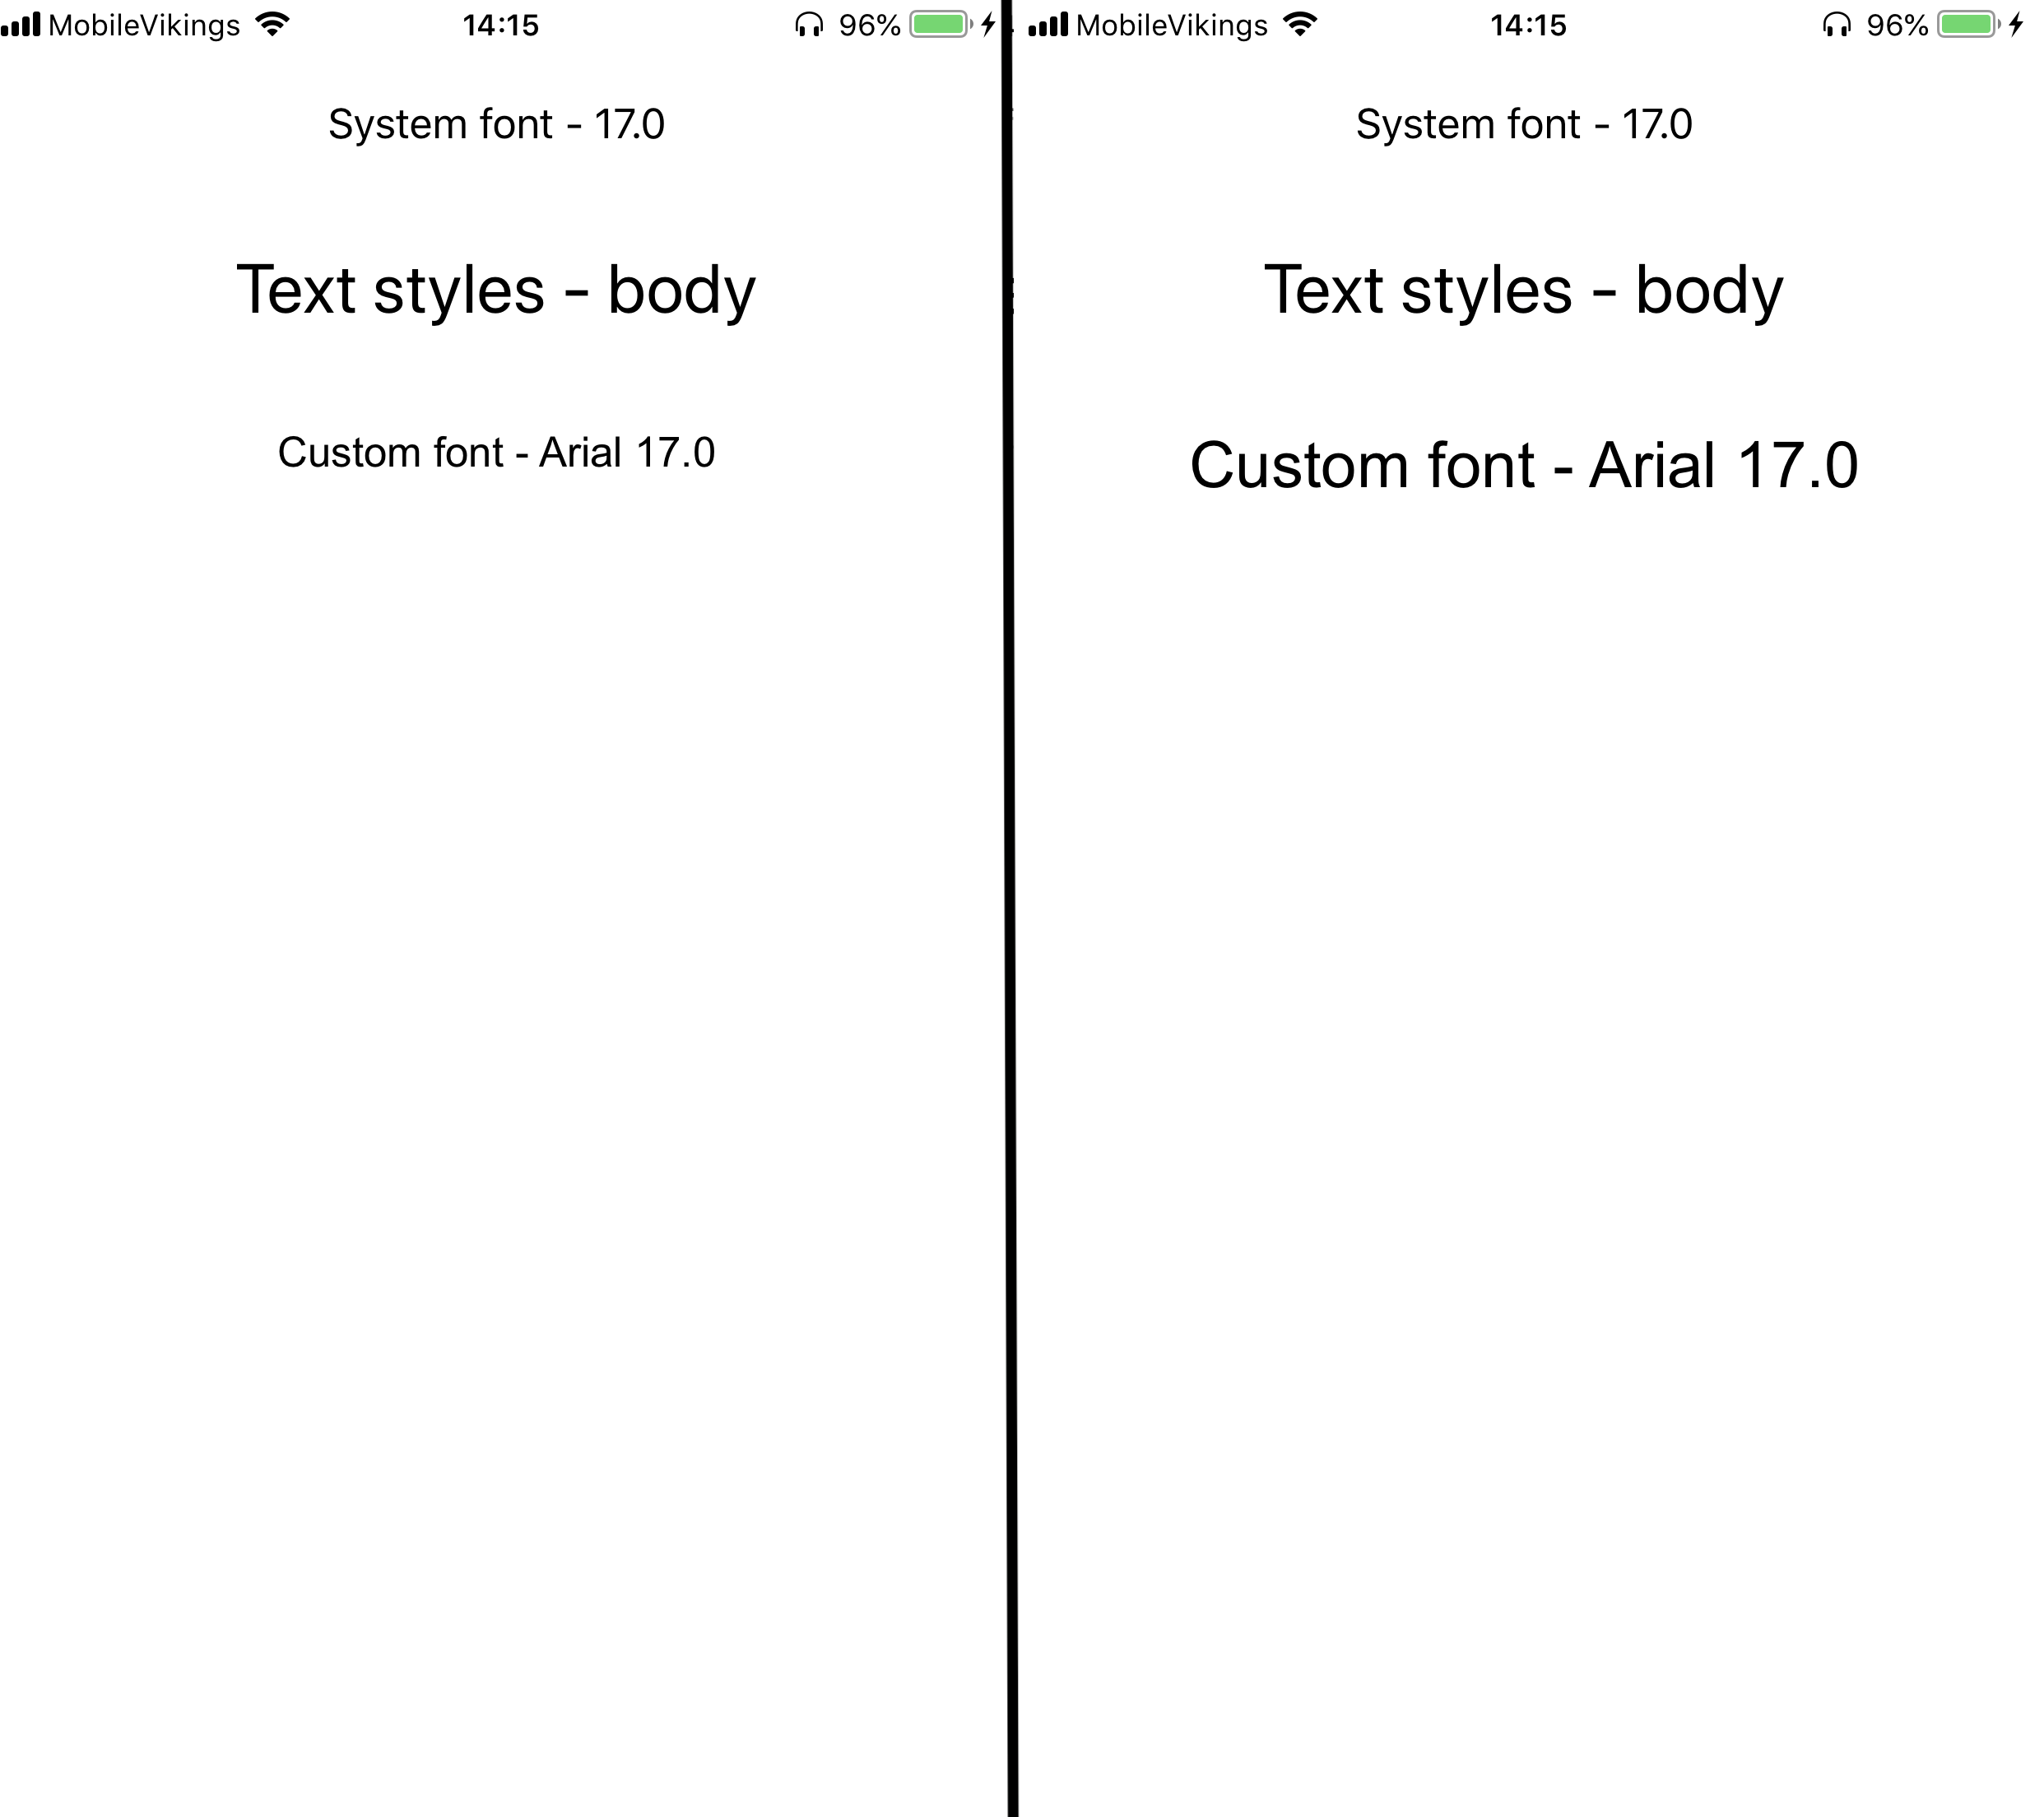
\includegraphics[width=0.7\linewidth]{img/iosFontCompare}}
    \caption{Voorbeeld vergroten tekst in iOS, links: custom lettertype niet schaalbaar, rechts: custom lettertype schaalbaar }
    \label{fig:iosFontCompare}
\end{figure}
\newpage
In figuur \ref{fig:iosFontCompare} is links de code uit voorbeeld \ref{dynamicTypeiOS} niet toegepast, het lettertype van type 'Custom' schaalt niet mee naar de wensen van de gebruiker. Rechts is de code uit voorbeeld \ref{dynamicTypeiOS} wel toegepast, de tekst schaalt mee.

Wanneer men een lettertype van de soort 'Text styles' gebruikt schaalt deze mee wanneer de applicatie opgestart wordt. Wanneer men dynamisch het lettertype wil schalen gedurende dat de applicatie actief is moet men de optie 'Automatically Adjusts Font' activeren. Deze optie kan gevonden worden in de 'Storyboard editor' in de 'Attribute inspector' van het corresponderende element.

\subsubsection{Verminderen transparantie}
Deze functionaliteit oogt op het verhogen van de leesbaarheid door transparantie te laten verdwijnen. Door de transparantie te laten verdwijnen verhoogt het contrast ook. In figuur \ref{fig:transparantieiOS} ziet u aan de linkerkant een voorbeeld van het besturingssysteem zonder dat de functionaliteit is geactiveerd. Aan de rechterkant is de functionaliteit geactiveerd, waarbij duidelijk te zien valt dat de transparantie minimaal is.
Een ontwikkelaar kan dankzij de property \emph{UIAccessibility.isReduceTransparencyEnabled} nagaan of deze functionaliteit is ingeschakeld. 
\begin{figure}[h]
    \centering
    \frame{ \includegraphics[width=0.7\linewidth]{img/transparantieiOS}}
    \caption{Voorbeeld verminderen transparantie in iOS, links: functionaliteit uit, rechts: functionaliteit aan}
    \label{fig:transparantieiOS}
\end{figure}
\newpage
\subsubsection{Verhogen contrast}
Deze functionaliteit maakt kleuren van elementen donkerder om een hogere contrast te krijgen. Afbeeldingen worden niet aangepast.
Een ontwikkelaar kan via de property \emph{UIAccessibility.isDarkerSystemColorsEnabled} nagaan of deze functionaliteit is ingeschakeld. 
\subsubsection{Vette tekst}
In iOS kan men met de functionaliteit 'Vette tekst' tekst beter leesbaar maken. Alle tekst wordt bij het inschakelen van deze functionaliteit omgezet naar vette tekst.
Via de property \emph{UIAccessibility.isBoldTextEnabled} kan men nagaan of deze functionaliteit is ingeschakeld. 
\subsection{Auditief}
\subsubsection{LED Flash voor notificaties}
Wanneer iemand deze functionaliteit ingeschakeld heeft zal bij een melding zal uit de flits van het toestel een reeks lichtflitsen maken. Deze functionaliteit kan gezien worden als een alternatief voor meldingen met geluid. Men heeft de optie om deze functionaliteit enkel te gebruiken wanneer het geluid van het toestel uit staat.
\subsubsection{Mono-geluid}
Wanneer iemand slechthorend is aan 1 kant kan het wenselijk zijn om beide audio kanalen te combineren naar 1 kanaal. Daardoor kan men alles horen, en mist men geen geluid omdat men maar 1 van de 2 kanalen kon horen. Dankzij deze functionaliteit wordt stereo-geluid aangepast naar mono-geluid.
Via de property \emph{UIAccessibility.isMonoAudioEnabled} kan men nagaan of deze functionaliteit is ingeschakeld.
\subsubsection{Kiezen van balans tussen linker en rechter audiokanaal}
Met deze functionaliteit kan gekozen worden aan de hand van een schuifknop welk audiokanaal men wilt horen. De audiokanalen worden NIET gecombineerd, men zal dus een deel van het afgespeelde geluid verliezen als men de functionaliteit 'Mono-geluid' niet inschakelt. 
\subsubsection{Ondertiteling}
\label{subsec:ondertiteliOS}
Dove of hardhorige mensen gebruiken ondertitelingen als alternatief op audio. Met het inschakelen van deze functionaliteit zullen ondertitelingen weergegeven worden wanneer deze beschikbaar zijn.

Deze functionaliteit is ook nog aanpasbaar naar de voorkeur van de gebruiker. Men kan de stijl van ondertitelingen aanpassen. Er zijn standaard 4 verschillende stijlen, maar die zijn uitbreidbaar met een eigen gemaakte stijl. Wanneer men een nieuwe stijl creëert kan men de tekstkleur, tekstgrootte en lettertype aanpassen. Ook kan de achtergrond en de doorzichtigheid aangepast worden. 

Vaak zullen video's hun vaste stijl gedefinieerd hebben voor ondertiteling, wanneer men een eigen gecreëerde stijl wilt gebruiken zal men  'Video overschrijven' moeten uitschakelen bij alle opties van de eigen gecreëerde stijl.

Een ontwikkelaar kan nagaan of een gebruiker ondertiteling heeft ingeschakeld via de property \emph{UIAccessibility.isClosedCaptioningEnabled}.

Raadpleeg de developer documentatie voor het toevoegen van ondertitelingen aan een AVMediaPlayer\footnote{\url{https://developer.apple.com/streaming/}}.
\subsection{Motorisch}
\subsubsection{Shortcut activatie toegankelijkheidsfunctionaliteiten}
Met deze functionaliteit kunnen personen met een motorische beperking, maar ook met andere beperkingen heel snel hun favoriete functionaliteit activeren. Bij het driemaal indrukken van de homeknop zal de functionaliteit die men geselecteerd heeft geactiveerd worden. Wanneer men meerdere functionaliteiten heeft geselecteerd zal een menu met deze functionaliteiten verschijnen.
\subsubsection{Switch Control}
Switch Control ook wel schakelbediening genoemd laat een gebruiker met een motorische beperking toe om te navigeren binnen iOS. Alle elementen op het scherm worden als het ware één voor één overlopen, waarbij men een element kan activeren door een schakel te gebruiken. Deze schakels kunnen extern zijn, maar kan ook komen vanuit het apparaat. De invoer vanuit het apparaat kunnen knoppen, maar ook touch gebaren zijn. Ook de camera van een apparaat kan gebruikt worden als switch, hierbij kijkt de camera naar bewegingen met het hoofd.

Switch Control is een functionaliteit die zeer aanpasbaar is. Men kan kiezen voor het groeperen van elementen voor snellere navigatie, of voor het afspelen van geluid bij het navigeren, etc.

Een ontwikkelaar kan aan de hand van de property \emph{UIAccessibility.isSwitchControlRunning} weten of iemand Switch Control gebruikt in zijn applicatie. Verder kunnen ontwikkelaars het navigeren in hun applicatie makkelijker maken door elementen te groeperen zoals dit gedaan werd in voorbeeld \ref{dynamicAccessVoiceOverGrouping}.
\subsubsection{AssistiveTouch}
AssistiveTouch maakt het mogelijk om een iOS-apparaat te bedienen zonder de fysieke knoppen te hoeven gebruiken. Bij het activeren van deze functionaliteit krijgt men een menu (AssistiveTouch-menu) op het scherm. Dit menu bevat iconen waarop men kan drukken, elk icoon heeft zijn corresponderende actie in iOS. Zo kan men bijvoorbeeld het scherm vergrendelen, het geluid verhogen, de homeknop bedienen, etc.

Naast het uitvoeren van acties waarvoor men de fysieke knoppen voor zou gebruiken kan men ook touch-gebaren toevoegen als een actie.  Deze gebaren worden dan uitgevoerd wanneer de actie geactiveerd wordt. Deze functionaliteit kan men zeer goed personaliseren, zo kan men kiezen hoeveel acties men in het menu wenst weer te geven. Of men kan 3D Touch gebruiken voor het activeren van een specifieke actie.  Maar ook de doorzichtigheid van het menu kan ingesteld worden.

Als ontwikkelaar kan men nagaan of deze functionaliteit is geactiveerd tijdens het gebruik van zijn applicatie via de volgende propery \emph{UIAccessibility.isAssistiveTouchRunning}.
\subsubsection{Aangepaste aanraking}

De functionaliteit 'Aangepaste aanraking' is een gecombineerde functionaliteit bestaande uit 3 verschillende functionaliteiten. Ze hebben alle 3 hetzelfde doel, namelijk het aanpassen van hoe het systeem reageert op aanrakingen. Voor onderstaande functionaliteiten te kunnen gebruiken moet men een schakelaar activeren.

De eerste functionaliteit is 'Vasthoudduur' waarbij men kan aanpassen hoelang men het scherm moet indrukken voor iOS het ziet als een aanraking op het touchscreen. Als men een aanraking doet maar men tilt de vinger op voor dat de ingestelde tijd is verstreken zal deze aanraking genegeerd worden. 


Met de functionaliteit 'Negeer herhaling' kan men instellen hoeveel tijd er tussen 2 aanrakingen moet zitten. Hoe langer de tijd die men instelt, hoe langer het besturingssysteem meerdere aanrakingen achter elkaar ziet als 1 aanraking.


De derde functionaliteit 'Tikassistentie' ondersteunt mensen met een motorische beperking die hun vingers ongewenst verplaatsen tijdens het aanraken van het scherm. Zonder deze functionaliteit kan men mogelijk een foutieve selectie maken. Men kan instellen dat iOS bij het aanraken van het scherm ofwel de laatste positie van de aanraking of de eerste positie registreert.

\subsection{Cognitief}
\subsubsection{Verminderen van bewegingen}
Een gebruiker kan met 'Verminderen van bewegingen' ervoor kiezen om animaties te vermijden binnen iOS. Bij het activeren van deze optie worden animaties van het besturingssysteem zelf verwijderd. In tegenstelling tot Android is dit niet het geval bij zelfontwikkelde applicaties.

\lstinputlisting[language=java,label=reduceMotioniOS, caption={Voorbeeld in Swift: Controleren of verminderen van bewegingen is ingeschakeld},frame=single, breaklines,basicstyle=\scriptsize, firstline=18,lastline=30]{../code/iOS/AnimationSample/AnimationSample/ViewController.swift}

Een ontwikkelaar zou bij het gebruik van animaties moeten controleren of een gebruiker deze functionaliteit heeft ingeschakeld. Indien dit het geval is moet de animatie vermeden worden. In voorbeeld \ref{reduceMotioniOS} wordt een animatie uitgevoerd als de optie \emph{UIAccessibility.isReduceMotionEnabled} niet is ingeschakeld.

\subsubsection{Begeleide toegang}
De functionaliteit 'Begeleide toegang' kan wanneer deze geactiveerd is voorkomen dat een gebruiker de applicatie sluit. Dit voorkomt dat een gebruiker afgeleid kan zijn. Enkel bij het ingeven van een wachtwoord, of het aanmelden met FaceID of TouchID kan de applicatie gesloten worden. Naast het voorkomen dat een applicatie gesloten kan worden, kan ook ingesteld worden door een gebruiker in welk gebied geen interactie mogelijk is. Daarnaast kunnen nog diverse zaken ingesteld worden bij het gebruik van een applicatie. Dit kan zijn:
\begin{itemize}
    \item Mogelijkheid tot sluimerknop te gebruiken
    \item Mogelijkheid tot gebruik volumeknoppen
    \item Mogelijkheid tot roteren van scherm
    \item Mogelijkheid tot gebruik toetsenbord
    \item Mogelijkheid tot aanraken van scherm
    \item Tijdslimiet (hoelang de applicatie mag gebruikt worden)
\end{itemize}

Deze functionaliteit kan wanneer deze is ingeschakeld in de instellingen, geactiveerd en gedeactiveerd worden door driemaal kort op de homeknop te drukken. Een ontwikkelaar kan detecteren als de functionaliteit is ingeschakeld in zijn applicatie via de volgende property: \emph{UIAccessibility.isGuidedAccessEnabled}. 

\lstinputlisting[language=java,label=iosAppIdentifierGuided, caption={Voorbeeld in Swift: AppDelegate met applicatie specifieke instellingen voor 'Begeleide toegang'},frame=single, breaklines,basicstyle=\scriptsize, firstline=12,lastline=26]{../code/iOS/GuidedAccess/GuidedAccess/AppDelegate.swift}

Een applicatie kan ook applicatie specifieke instellingen hebben. Deze kunnen bij het activeren van de functionaliteit in de applicatie aan- of uitgezet worden. Met deze instellingen kunnen bepaalde onderdelen van de applicatie geblokkeerd worden, bijvoorbeeld: Toegang tot online wedstrijden in een spelletje.  In voorbeeld \ref{iosAppIdentifierGuided} wordt een applicatie specifieke instelling gedefinieerd. Dit is mogelijk gemaakt door het invullen van de methodes die  overgeërfd werden van het protocol \emph{UIGuidedAccessRestrictionDelegate} in de AppDelegate . De methode \emph{guidedAccessRestrictionIdentifiers} bevat een lijst met alle applicatie specifieke instellingen die men wilt toevoegen. De methode \emph{detailTextForGuidedAccessRestriction(withIdentifier restrictionIdentifier: String)} retourneert voor elke instelling een bijpassende naam. Deze naam is zichtbaar in het instellingen menu.

In voorbeeld \ref{iosAppIdentifierGuidedReaction} wordt een methode gedefinieerd die ook overgeërfd is in de AppDelegate. Deze methode is: \emph{guidedAccessRestriction(withIdentifier restrictionIdentifier: String, didChange newRestrictionState: UIAccessibility.GuidedAccessRestrictionState)}. Met deze methode kan nagegaan worden of een applicatie specifieke instelling geactiveerd werd. Indien dit het geval is kan men dit verder behandelen in de applicatie.
\newpage
\lstinputlisting[language=java,label=iosAppIdentifierGuidedReaction, caption={Voorbeeld in Swift: AppDelegate met methode voor nagaan of applicatie specifieke instelling voor 'Begeleide toegang' werd geactiveerd.'},frame=single, breaklines,basicstyle=\scriptsize, firstline=28,lastline=44]{../code/iOS/GuidedAccess/GuidedAccess/AppDelegate.swift}
%\lipsum[76-80]
\section{Verschillen/gelijkenissen in functionaliteiten Android en iOS}
Uit de bespreking van de toegankelijkheidsfunctionaliteiten in secties \ref{sec:ToegankelijkheidsfunctionaliteitenAndroid} en \ref{sec:ToegankelijkheidsfunctionaliteiteniOS} blijkt,  dat zowel Android als iOS een zeer uitgebreide set aan functionaliteiten bezit. Er kan niet duidelijk gesteld worden dat een besturingssysteem primeert, dit komt vooral door de gelijkenissen en verschillen tussen beide platformen. Wel kan er gesteld worden dat het aantal standaard meegeleverde functionaliteiten kleiner is in Android dan in iOS. In Android is dan weer de mogelijkheid om toegankelijkheidsfunctionaliteiten te downloaden en te ontwikkelen. In de bespreking van de functionaliteiten werden de meest relevante besproken. De virtuele assistenten 'Google Assistant' en 'Siri' werden buiten beschouwing gelaten.


In tabel \ref{overzichtFunctionaliteitenBesproken} vindt u een overzicht met de besproken functionaliteiten. Ook wordt het verschil ten opzichte van functionaliteiten duidelijk gemaakt. Duidelijk zichtbaar is dat de meeste functionaliteiten beschikbaar zijn op beide besturingssystemen. Bij Android werden enkel de standaardfunctionaliteiten besproken. Sommige smartphones met Android kunnen nog extra standaard meegeleverde functionaliteiten bevatten. iOS heeft niet de mogelijkheid om extra functionaliteiten toe te voegen, maar het besturingssysteem bevat wel een brede basis. 

Zowel Android als iOS laten ontwikkelaars toe om toegankelijkheidsfunctionaliteiten te faciliteren in hun applicaties. iOS geeft de ontwikkelaar veel inzicht in welke functionaliteiten ingeschakeld zijn. Wat minder vanzelfsprekend is in Android. Opvallend is dat het schaalbaar maken van tekst veel omslachtiger is in iOS dan in Android. 

\begin{table}
    \centering
    \caption{Overzicht besproken functionaliteiten in Android en iOS per domein}
    \label{overzichtFunctionaliteitenBesproken}
    \begin{tabular}{|l|l|l|} 
        \hline
        \multicolumn{3}{|l|}{\textbf{Visueel} }                                                        \\ 
        \hline
        \textbf{Beschrijving}                                 & \textbf{Android}  & \textbf{iOS}       \\ 
        \hline
        Navigeren via audio feedback                          & TalkBack          & VoiceOver          \\ 
        \hline
        Schalen van lettertypes                               & Ja                & Ja                 \\ 
        \hline
        Schalen van weergave grootte~                         & Ja                & Nee                \\ 
        \hline
        Inzoomen op elementen                                 & Ja                & Ja                 \\ 
        \hline
        Filters voor kleurenblindheid                         & Ja                & Ja                 \\ 
        \hline
        Verhogen contrast~                                    & Ja                & Ja                 \\ 
        \hline
        Inverteren kleuren                                    & Ja                & Ja                 \\ 
        \hline
        Vette tekst                                           & Nee~              & Ja                 \\ 
        \hline
        \multicolumn{3}{|l|}{}                                                                         \\ 
        \hline
        \multicolumn{3}{|l|}{\textbf{Auditief}}                                                        \\ 
        \hline
        \textbf{Beschrijving}                                 & \textbf{Android~} & \textbf{iOS}       \\ 
        \hline
        Mono-geluid                                           & Ja                & Ja                 \\ 
        \hline
        (Aanpasbare) ondertiteling                            & Ja                & Ja                 \\ 
        \hline
        Geluidsversterker                                     & Ja                & Beperkt            \\ 
        \hline
        LED flash voor notificaties                           & Nee               & Ja                 \\ 
        \hline
        \multicolumn{3}{|l|}{}                                                                         \\ 
        \hline
        \multicolumn{3}{|l|}{\textbf{Motorisch}}                                                       \\ 
        \hline
        \textbf{Beschrijving}                                 & \textbf{Android}  & \textbf{iOS}       \\ 
        \hline
        Hardware knoppen voor besturen                        & Ja                & Ja                 \\ 
        \hline
        Scherm automatisch draaien                            & Ja                & Ja                 \\ 
        \hline
        Vertragingen bij aanraken                             & Ja                & Ja                 \\ 
        \hline
        Hardware activatie van functionaliteiten              & Ja                & Ja                 \\ 
        \hline
        Vervanging van hardware knoppen                       & Nee               & AssistiveTouch     \\ 
        \hline
        \multicolumn{3}{|l|}{}                                                                         \\ 
        \hline
        \multicolumn{3}{|l|}{\textbf{Cognitief}}                                                       \\ 
        \hline
        \textbf{Beschrijving}                                 & \textbf{Android}  & \textbf{iOS}       \\ 
        \hline
        Verwijderen van animaties                             & Ja                & Ja                 \\ 
        \hline
        Beperken van afleiding bij gebruik van een applicatie & Nee               & Begeleide toegang  \\
        \hline
    \end{tabular}
\end{table}
\chapter{\IfLanguageName{dutch}{Richtlijnen voor mobiele applicaties}{Richtlijnen voor  mobiele applicaties}}
\label{ch:Richtlijnen voor toegankelijkheid mobiele applicaties}
Een ontwikkelaar moet kunnen nagaan of zijn mobiele applicatie toegankelijk is. De bestaande richtlijnen zijn intimiderend. En men kan moeilijk toetsen wanneer men voldaan heeft. In dit hoofdstuk wordt aan de hand van de WCAG richtlijnen een maatstaf opgesteld voor ontwikkelaars. Hierdoor kan vlot een inzicht gecreëerd worden over de toegankelijkheid van een mobiele applicatie.

\section{WCAG richtlijnen}
\label{sec:WCAGrichtlijn}

Zoals reeds besproken is in sectie \ref{sec:wetgeving} vormen de WCAG richtlijnen de basis voor dit onderzoek. Meer bepaald de richtlijnen die besproken zijn in WCAG 2.1. Deze richtlijnen bevatten extra criteria gericht op het gebruik van touchscreens, visuele beperkingen en cognitieve beperkingen.
De succescriteria beschreven in de WCAG richtlijnen zijn technologie onafhankelijk opgesteld. Dit wil zeggen dat ze zowel op mobiele platformen als computers kunnen toegepast worden. Vaak wordt het woord 'web' gebruikt in een richtlijn, wat in de meeste gevallen vervangen kan worden door 'mobiele applicatie'.
 \autocite{w3cTechnologyNeutral}

De WCAG 2.1 richtlijnen zijn opgebouwd in een specifieke structuur. De richtlijnen en de daarbij horende succescriteria zijn onderverdeeld onder vier verschillende principes. Aan deze principes moet voldaan worden om een toegankelijke applicatie te hebben. Deze principes zijn respectievelijk: 
\begin{itemize}
    \item Waarneembaar: gebruikers moeten de informatie (op het scherm) kunnen waarnemen.
        \item Bedienbaar: gebruikers moeten kunnen de elementen kunnen bedienen, waaronder ook navigatie.
        \item Begrijpelijk: gebruikers moeten de informatie en bediening van een applicatie verstaan.
        \item Robuust: gebruikers moeten de inhoud blijven kunnen gebruiker wanneer ze nieuwe technologie gebruiken.
\end{itemize}

Binnen de principes zijn er richtlijnen. Deze richtlijnen bevatten de doelen die men moet behalen voor aan een principe te voldoen. Die doelen kunnen behaald worden door de applicatie te toetsen aan succescriteria. Een succescriteria schrijft vereisten voor waaraan voldaan moet worden om een richtlijn te kunnen behalen. 

Elk succescriteria bevat een niveau, deze niveaus komen overeen met de afstemming op de behoeften van gebruikers met een beperking. Deze levels zijn:
\begin{itemize}
    \item Niveau A: Minimum level, voldoet aan niveau A succescriteria.
    \item Niveau AA: Voldoet aan niveau A succescriteria en niveau AA succescriteria.
    \item Niveau AAA: Voldoet aan niveau A, AA en AAA succescriteria.
\end{itemize}

Binnen dit onderzoek zullen wij ons focussen op niveau A en niveau AA succesfactoren. De WCAG richtlijnen raden af om alle succescriteria te proberen afstemmen tot niveau AAA. Ze vermelden dat het onmogelijk is om deze allemaal te behalen. 

Als voorbeeld:  \emph{Succesfactor 1.2.6: Er wordt een gebarentaalvertolking geleverd voor alle vooraf opgenomen audiocontent in gesyncroniseerde media. (Level AAA)}. Er kan gesteld worden, dat dit onmogelijk is voor vele applicaties om daaraan te voldoen \autocite{WCAG2.1Criteria}.

In het vervolg van deze sectie gaan wordt per principe de richtlijnen en succesfactoren bespreken. Om een indruk te kunnen geven van de potentiële impact op de gebruikers van een succesfactor wordt er een score aan toegekend. Deze score drukt de potentiële impact uit op de gebruikservaring van de app (of een specifieke functionaliteit ervan) voor een van de 4 (ruim gedefinieerde) doelgroepen.
Hoe hoger de score, hoe aannemelijker het is dat een correcte toepassing van dit WCAG-criterium een bovengemiddelde impact heeft op de gebruikerservaring. De scores hebben de volgende betekenis:
\begin{enumerate}
    \item Geen bovengemiddelde impact
    \item Bovengemiddelde impact
    \item Essentiële impact
\end{enumerate}

\newpage
\subsection{Principe 1: Waarneembaar}
\label{sec:waarneembaarWCAG}
Dit principe stelt dat informatie en elementen van een applicatie gepresenteerd moeten worden zodanig dat men die kan waarnemen.


\subsubsection{Richtlijn 1.1 - Tekst alternatieven}
Gebruikers kunnen nood hebben aan een alternatief voor inhoud die geen tekst bevat. Voor deze richtlijn te faciliteren moet aan de succesfactoren in tabel xx voldaan worden.
\begin{table}[H]
    \centering
 \hspace*{-1cm}\begin{tabular}{|l|p{12cm}|} 
        \hline
        \textbf{Succesfactor}                & 1.1.1                                                                                                                                                                                                                                                                                                             \\ 
        \hline
        \textbf{Level}                       & A                                                                                                                                                                                                                                                                                                                                                                             \\ 
        \hline
        \textbf{Naam}                        & Niet-tekst inhoud~                                                                                                                                                                                                                                                                                                                                                            \\ 
        \hline
        \textbf{Slagen van succesfactor}     & \begin{itemize}
            \item Tekstalternatieven voorzien voor niet-tekst inhoud (bv. afbeeldingen, knoppen, …)
        \end{itemize}                                                                                                                                                                                                      \\ 
        \hline
        \textbf{Beschrijving}                & Vooral gebruikers met een visuele beperking zullen gebruik maken van VoiceOver of TalkBack. Ze besturen hun smartphone via audio feedback. Alle elementen die tekst bevatten worden voorgelezen. Sommige elementen bevatten geen of weinig betekenisvolle tekst. Men moet dus goede tekst alternatieven voorzien voor niet-tekst inhoud.  \\ 
        \hline
        \textbf{Impact op gebruikers}        & 
        \begin{itemize}
            \item Visueel: 3, verhoogt het waarnemen van inhoud.
            \item Cognitief: 2, maakt makkelijker om inhoud op te nemen.             
        \end{itemize}                                                                                                                   \\ 
        \hline
        \textbf{Platform specifieke feature} & \begin{itemize}
            \item iOS: VoiceOver, zie \ref{subsec:VoiceOver}.
            \item Android: TalkBack, zie \ref{subsec:TalkBack}
        \end{itemize}                                                                                                                                                                       \\ 
        \hline
        \textbf{Testen}                      & Deze succesfactor kan getest worden door een ontwikkelaar met ofwel TalkBack of VoiceOver de mobiele applicatie te besturen. Wanneer een element niet duidelijk benoemd is (voornamelijk afbeeldingen), kan gesteld worden dat er niet voldaan wordt aan het succescriteria.                                                                                                                                                                                                                        \\
        \hline
    \end{tabular}
\end{table}



%\paragraph{Succesfactor 1.1.1: Niet-tekst inhoud (A)}
%Vooral gebruikers met een visuele beperking zullen gebruik maken van VoiceOver of TalkBack. Ze besturen hun smartphone via audio feedback. Alle elementen die tekst bevatten worden voorgelezen. Sommige elementen bevatten geen of weinig betekenisvolle tekst. Men moet dus goede tekst alternatieven voorzien voor niet-tekst inhoud. Zie sectie \ref{subsec:TalkBack} en \ref{subsec:VoiceOver} voor details over de implementatie. Om te voldoen aan deze succesfactor moet een men: 
%\begin{itemize}
  %  \item Tekstalternatieven voorzien voor niet-tekst inhoud (bv. afbeeldingen, knoppen, ...)
%\end{itemize}
%Een succesvolle implementatie van de succesfactor biedt voordeel aan:
%\begin{itemize}
%    \item Visuele beperking: moeilijkheden met waarnemen beeld.
%    \item Cognitieve beperking: moeilijkheden met opnemen betekenis van elementen (bv. foto's)
%\end{itemize}
%Deze succesfactor kan getest worden dooreen ontwikkelaar met ofwel TalkBack of VoiceOver de mobiele applicatie te besturen. Wanneer een element niet duidelijk benoemd is (voornamelijk afbeeldingen), kan gesteld worden dat er niet voldaan wordt aan het succescriteria.
\subsubsection{Richtlijn 1.2: Tijds-gebaseerde media}
Gebruikers moeten een alternatief hebben voor tijds-gebaseerde media. Dit is zowel vooraf opgenomen media als live media. 
\newpage
\begin{table}[H]
    \centering
    \hspace*{-1cm}\begin{tabular}{|l|p{12cm}|} 
        \hline
        \textbf{Succesfactor}                & 1.2.1                                                                                                                                                                                                                                                                                                             \\ 
        \hline
        \textbf{Level}                       & A                                                                                                                                                                                                                                                                                                                                                                             \\ 
        \hline
        \textbf{Naam}                        & Vooraf opgenomen geluid of beeld~                                                                                                                                                                                                                                                                                                                                                            \\ 
        \hline
        \textbf{Slagen van succesfactor}     & \begin{itemize}
            \item Bij enkel audio: een tekst transcript voorzien.
            \item Bij enkel video: een audio fragment of tekst transcript voorzien.
        \end{itemize}                                                                                                                                                                                                      \\ 
     \hline
    \textbf{Uitzonderingen}     & \begin{itemize}
        \item Wanneer de media een alternatief is voor tekst (die aanwezig is), hoeft er geen rekening gehouden te worden voor dat media element.
    \end{itemize}                                                                                                                                                                                                      \\ 
        \hline
        \textbf{Beschrijving}                & Wanneer men te maken heeft met inhoud die ofwel geluid of beeld moet een alternatief voorzien worden. Bij bijvoorbeeld een audio is een transcriptie die beschrijft wat er gebeurt gewenst. Bij video is een transcriptie of een audio track die beschrijft wat er te horen valt gewenst. \\ 
        \hline
        \textbf{Impact op gebruikers}        & 
        \begin{itemize}
            \item Visueel: 3, verhoogt het waarnemen van inhoud (bij beeld).
            \item Auditief 3, verhoogt waarnemen van inhoud (bij geluid).             
        \end{itemize}                                                                                                                   \\ 
        \hline
        \textbf{Testen}                      & Men kan nagaan of voldaan wordt aan de richtlijn, wanneer men er niet in slaagt, kan gesteld worden dat men niet voldoet aan de richtlijn.                                                                                                                                                                                                            \\
        \hline
    \end{tabular}
\end{table}
\begin{table}[H]
    \centering
    \hspace*{-1cm}\begin{tabular}{|l|p{12cm}|} 
        \hline
        \textbf{Succesfactor}                & 1.2.2                                                                                                                                                                                                                                                                                                             \\ 
        \hline
        \textbf{Level}                       & A                                                                                                                                                                                                                                                                                                                                                                             \\ 
        \hline
        \textbf{Naam}                        & Ondertitelingen bij vooraf opgenomen video’s met audio~                                                                                                                                                                                                                                                                                                                                                            \\ 
        \hline
        \textbf{Slagen van succesfactor}     & \begin{itemize}
            \item Ondertitelingen toevoegen aan video’s waar geluid is.
        \end{itemize}                                                                                                                                                                                                      \\ 
        \hline
        \textbf{Uitzonderingen}     & \begin{itemize}
            \item Wanneer de video een alternatief is voor tekst (die aanwezig is), hoeft er geen rekening gehouden te worden met de succesfactor.
        \end{itemize}                                                                                                                                                                                                      \\ 
        \hline
        \textbf{Beschrijving}                & Ondertitelingen worden vaak gebruikt bij gebruikers met een auditieve beperking. Het biedt een tekstalternatief voor de audio die afgespeeld wordt in een video. \\ 
        \hline
        \textbf{Impact op gebruikers}        & 
        \begin{itemize}
            \item Auditief 3, verhoogt waarnemen van inhoud.             
        \end{itemize}                                                                                                                   \\ 
      \hline
    \textbf{Platform specifieke feature} & \begin{itemize}
        \item iOS: zie \ref{subsec:ondertiteliOS}.
        \item Android: zie \ref{subsec:ondertitelAndroid}
    \end{itemize}                                                                                                                                                                       \\ 
        \hline
        \textbf{Testen}                      & Men kan nagaan of voldaan wordt aan de richtlijn. Wanneer een video, die niet dient als alternatief voor een tekst, geen ondertitelingen ondersteunt, kan gesteld worden dat er niet voldaan wordt.                                                                                                                                                                                              \\
        \hline
    \end{tabular}
\end{table}





%\paragraph{Succesfactor 1.2.1: Vooraf opgenomen geluid of beeld (A)}
%Wanneer men te maken heeft met inhoud die ofwel geluid of beeld moet een alternatief voorzien worden. Bij bijvoorbeeld een audio is een transcriptie die beschrijft wat er gebeurt gewenst. Bij video is een transcriptie of een audio track die beschrijft wat er te horen valt gewenst. Om te voldoen aan deze succesfactor moet men: \begin{itemize}
   % \item Bij enkel audio: een tekst transcript voorzien.
    %\item Bij enkel video: een audio fragment of tekst transcript voorzien.
%\end{itemize}
%Een succesvolle implementatie van de succesfactor biedt voordeel aan:
%\begin{itemize}
    %\item Visuele beperking: moeilijkheden met waarnemen beeld.
  %  \item Auditieve beperking: moeilijkheden waarnemen van geluiden.
%\end{itemize}
%Wanneer de media een alternatief is, bijvoorbeeld voor visuele representatie van een tekst, hoeft geen rekening gehouden te worden met de succesfactor. 
\begin{table}[H]
    \centering
    \hspace*{-1cm}\begin{tabular}{|l|p{12cm}|} 
        \hline
        \textbf{Succesfactor}                & 1.2.3                                                                                                                                                                                                                                                                                                             \\ 
        \hline
        \textbf{Level}                       & A                                                                                                                                                                                                                                                                                                                                                                             \\ 
        \hline
        \textbf{Naam}                        & Audiodescriptie of alternatief bij vooraf opgenomen video’s met audio~                                                                                                                                                                                                                                                                                                                                                            \\ 
        \hline
        \textbf{Slagen van succesfactor}     & \begin{itemize}
            \item Een audio beschrijving te voorzien voor video’s, of
            \item een volledig transcript van de video voorzien.
        \end{itemize}                                                                                                                                                                                                      \\ 
        \hline
        \textbf{Uitzonderingen}     & \begin{itemize}
            \item Wanneer de video een alternatief is voor tekst (die aanwezig is), hoeft er geen rekening gehouden te worden met de succesfactor.
        \end{itemize}                                                                                                                                                                                                      \\ 
        \hline
        \textbf{Beschrijving}                & Gebruikers met een visuele een beperking wensen graag een beschrijving van wat er gebeurt in een video. Een audiodescriptie geeft deze gebruikers via geluid uitleg wat er te zien valt in de video. Dit kan gebeuren via een audio descriptie, of een transcript te voorzien. Dit transcript kan door de screenreader dan voorgelezen worden.\\ 
        \hline
        \textbf{Impact op gebruikers}        & 
        \begin{itemize}
            \item Visueel 3, verhoogt waarnemen van inhoud.    
            \item Cognitief 2, verhoogt verstaanbaarheid bewegende beelden         
        \end{itemize}                                                                                                                   \\ 
      
        \hline
        \textbf{Testen}                      & Men kan nagaan of voldaan wordt aan de richtlijn. Wanneer een video, die niet dient als alternatief voor een tekst, een audio beschrijving heeft, of een transcript van de audio voorzien is. Dan slaagt men met het implementeren van deze succesfactor.                                                                                                                               \\
        \hline
    \end{tabular}
\end{table}




%\paragraph{Succesfactor 1.2.2: Ondertitelingen bij vooraf opgenomen video's met audio (A)}
%Ondertitelingen worden vaak gebruikt bij gebruikers met een auditieve beperking. Het biedt een tekstalternatief voor de audio die afgespeeld wordt in een video. Om te voldoen aan deze succesfactor dient men: 
%\begin{itemize}
%    \item Ondertitelingen toe te voegen aan video's waar geluid is.
%\end{itemize}
%Ook bij deze succesfactor geldt dat wanneer de video een alternatief is voor reeds bestaande tekst, men geen rekening hoeft te houden ermee.

%Een succesvolle implementatie van de succesfactor biedt voordeel aan:
%\begin{itemize}
%    \item Auditieve beperking: moeilijkheden waarnemen van geluiden.
%\end{itemize}
%Zie sectie \ref{subsec:ondertitelAndroid} en \ref{subsec:ondertiteliOS} voor de implementatie/functionaliteit van ondertitelingen in Android en iOS. 
%\paragraph{Succesfactor 1.2.3: Audiodescriptie of alternatief bij vooraf opgenomen video's met audio (A)}
%Gebruikers met een visuele een beperking wensen graag een beschrijving van wat er gebeurt in een video. Een audiodescriptie geeft deze gebruikers via geluid uitleg wat er te zien valt in de video.
%Dit kan gebeuren via een audio descriptie, of een transcript te voorzien. Dit transcript kan door de screenreader dan voorgelezen worden.
%Om te voldoen aan deze succesfactor dient men: 
%\begin{itemize}
%%    \item Een audio beschrijving te voorzien voor video's, of
 %      \item een transcript van de audio voorzien voor video's te voorzien.
    
%\end{itemize}
%Men hoeft geen rekening te houden met deze succesfactor wanneer de video een %alternatief is voor een tekst.

%Een succesvolle implementatie van de succesfactor biedt voordeel aan:
%\begin{itemize}
%    \item Visuele beperking: moeilijkheden waarnemen van beeld.
%        \item Cognitieve beperking: moeilijkheden verstaan van bewegende beelden.
%\end{itemize}

\begin{table}[H]
    \centering
    \hspace*{-1cm}\begin{tabular}{|l|p{12cm}|} 
        \hline
        \textbf{Succesfactor}                & 1.2.4                                                                                                                                                                                                                                                                                                             \\ 
        \hline
        \textbf{Level}                       & AA                                                                                                                                                                                                                                                                                                                                                                             \\ 
        \hline
        \textbf{Naam}                        & Ondertitelingen bij live video’s met audio~                                                                                                                                                                                                                                                                                                                                                            \\ 
        \hline
        \textbf{Slagen van succesfactor}     & \begin{itemize}
            \item Ondertitelingen toevoegen aan live video’s waar geluid is.
        \end{itemize}                                                                                                                                                                                                      \\ 
        \hline
        \textbf{Beschrijving}                & Gebruikers met een auditieve beperking hebben vooral baat bij het gebruik van ondertite- lingen in een live video met geluid.  \\ 
        \hline
        \textbf{Impact op gebruikers}        & 
        \begin{itemize}
            \item Auditief 3, verhoogt waarnemen van inhoud.             
        \end{itemize}                                                                                                                   \\ 
        \hline
        \textbf{Platform specifieke feature} & \begin{itemize}
            \item iOS: zie \ref{subsec:ondertiteliOS}.
            \item Android: zie \ref{subsec:ondertitelAndroid}
        \end{itemize}                                                                                                                                                                       \\ 
        \hline
        \textbf{Testen}                      & Elke live video met geluid moet ondertitelingen bevatten bij het activeren ervan.                                                                                                                                                                                    \\
        \hline
    \end{tabular}
\end{table}

\paragraph{Succesfactor 1.2.4: Ondertitelingen bij live video's met audio (AA)}
Gebruikers met een auditieve beperking hebben vooral baat bij het gebruik van ondertitelingen in een live video met geluid. Om te voldoen aan deze succesfactor moet men: 
\begin{itemize}
    \item Ondertitelingen toevoegen aan live video's waar geluid is.
\end{itemize}
Een succesvolle implementatie van de succesfactor biedt voordeel aan:
\begin{itemize}
    \item Auditieve beperking: moeilijkheden waarnemen van geluiden.
\end{itemize}

Zie sectie \ref{subsec:ondertitelAndroid} en \ref{subsec:ondertiteliOS} voor de implementatie/functionaliteit van ondertitelingen in Android en iOS. 

\paragraph{Succesfactor 1.2.5: Audiodescriptie bij vooraf opgenomen video's met audio (AA)}
Deze succesfactor leunt sterk aan tegen succesfactor 1.2.3. Deze overlapping komt doordat men in 1.2.5 (niveau AA) iets hogere vereisten stelt. 
In 1.2.3 heeft men de keuze voor een transcript, of een audiodescriptie te voorzien. In 1.2.5 wordt men verplicht om een audiodescriptie te voorzien. 

Om te voldoen aan deze succesfactor dient men: 
\begin{itemize}
    \item Een audio beschrijving te voorzien voor video's.
    
\end{itemize}
Men hoeft geen rekening te houden met deze succesfactor wanneer de video een alternatief is voor een tekst.

Een succesvolle implementatie van de succesfactor biedt voordeel aan:
\begin{itemize}
    \item Visuele beperking: moeilijkheden waarnemen van beeld.
    \item Cognitieve beperking: moeilijkheden verstaan van bewegende beelden.
\end{itemize}

\subsubsection{Richtlijn 1.3 - Aanpasbaar}
Deze richtlijn focust op het feit dat alle informatie beschikbaar is in de vorm waarin hij kan waargenomen worden. Bijvoorbeeld door het gebruik van VoiceOver of TalkBack. Daarvoor moet de informatie in een applicatie kunnen waargenomen worden door die software.
\paragraph{Succesfactor 1.3.1:  Informatie en relaties tussen informatie (A)}
Een gebruiker die gebruik maakt van een screenreader voor te navigeren. Alle informatie op het scherm moet daarvoor kunnen bepaald worden door die software. Voor deze succesfactor te implementeren dient:
\begin{itemize}
    \item Alle informatie waarneembaar te zijn door een screenreader.
\end{itemize}
Een succesvolle implementatie van de succesfactor biedt voordeel aan:
\begin{itemize}
    \item Visuele beperking: elementen op scherm worden correct voorgelezen.
\end{itemize}
Zie sectie \ref{subsec:TalkBack} en \ref{subsec:VoiceOver} voor details over de implementatie.

\paragraph{Succesfactor 1.3.2:  Betekenisvolle volgorde (A)}
Bij het gebruik van een screenreader kan volgorde van de informatie vaak van belang zijn. Een gebruiker met een visuele beperking, voornamelijk blinden zullen moeite hebben met de context van de informatie. Wanneer deze niet logisch gerangschikt, gegroepeerd staat, kan dit problemen geven.
Om deze succesfactor succesvol te implementeren dient:
\begin{itemize}
    \item De inhoud logisch geordend zijn.
    \item Gerelateerde informatie gegroepeerd staan.
\end{itemize}
Een succesvolle implementatie van de succesfactor biedt voordeel aan:
\begin{itemize}
    \item Visuele beperking: elementen op scherm worden correct voorgelezen.
\end{itemize}
Zie sectie \ref{subsec:TalkBack} en \ref{subsec:VoiceOver} voor details over hoe men inhoud logisch kan groeperen binnen een applicatie.
\paragraph{Succesfactor 1.3.3:  Zintuiglijke eigenschappen (A)}
Deze succesfactor verhindert dat gebruikers met een visuele beperking een mobiele applicatie niet kunnen bedienen door onduidelijke instructies. Bijvoorbeeld: een blinde gebruiker zal niks zijn met de instructie om op de derde knop links te drukken. Voor zo'n actie uit te voeren mag men niet blind zijn. 

Hetzelfde voor mensen met een auditieve beperking, wanneer instructies enkel via geluid worden gegeven, kan deze gebruiker geen actie ondernemen.

Om deze succesfactor succesvol te implementeren dient men: 
\begin{itemize}
    \item Instructies te geven die waarneembaar zijn voor verschillende zintuigen (visueel, auditief, ...)
\end{itemize}

Men kan in iOS eventueel inspelen als developer op de properties in de klasse \emph{UIAccessibility}. In Android kan men van bepaalde instellingen de waarden opvragen. 
Een succesvolle implementatie van de succesfactor biedt voordeel aan mensen met een:
\begin{itemize}
    \item Visuele beperking
    \item Auditieve beperking
\end{itemize}

\paragraph{Succesfactor 1.3.4:  Oriëntatie scherm (AA)}
Een smartphone kan gebruikt worden in portret- of landschapmodus. Men kan wisselen van modus door het apparaat te roteren. 
Gebruikers met een motorische beperking zullen vaak niet de mogelijkheid hebben om te wisselen van modus. Daarom stelt deze succesfactor dat de inhoud van een mobiele applicatie hetzelfde moet zijn in zowel portret- als landschapmodus.

Om te voldoen aan deze succesfactor dient:
\begin{itemize}
    \item Alle informatie en functionaliteiten identiek zijn in zowel portet- als landschapmodus.
\end{itemize}

Een ontwikkelaar moet rekening houden met de mogelijkheid tot roteren van het scherm bij het ontwikkelen van de applicatie. Wanneer men de lay-out opmaakt dient men hier aandacht aan te besteden.

Een succesvolle implementatie van de succesfactor biedt voordeel aan mensen met een motorische beperking.

\paragraph{Succesfactor 1.3.5:  Identificeerbaar doel van invoerveld (AA)}
Wanneer men een formulier of veld moet invullen moet elk veld een duidelijk identificeerbaar doel hebben. Dit kan zijn door het gebruik van labels, maar ook door de juiste metadata aan een veld te geven.
Wanneer metadata toegevoegd is, kan het besturingssysteem eventueel aanbevelingen geven aan de gebruiker welke informatie ingevuld moet worden.

Om te voldoen aan deze succesfactor dient men:
\begin{itemize}
    \item Aan elk veld een duidelijk doel te koppelen.
\end{itemize}

Voor aan deze succesfactor te voldoen kan men dus kiezen voor duidelijke labels, en eventueel metadata te koppelen aan velden. Binnen iOS kan men gebruik maken van \emph{Text input traits}, in Android kan men een \emph{inputType} koppelen aan een element.

Een succesvolle implementatie van de succesfactor biedt voordeel aan mensen met een:
\begin{itemize}
    \item Cognitieve beperking: moeilijkheden met taal, of geheugen
    \item Motorische beperking: moeite met invullen van velden
    \item Visuele beperking: duidelijkere beschrijving verwachte input (screenreader)
\end{itemize}

\subsubsection{Richtlijn 1.4 - Onderscheidbaar}
https://www.wuhcag.com/images-of-text/
\paragraph{Succesfactor 1.4.1:  Gebruik van kleur (A)}
\paragraph{Succesfactor 1.4.2:  Controle over geluid (A)}
\paragraph{Succesfactor 1.4.3:  Contrast (Minimum) (AA)}
\paragraph{Succesfactor 1.4.4:  Schalen van tekst (AA)}
\paragraph{Succesfactor 1.4.5:  Tekst in een afbeelding (AA)}
\paragraph{Succesfactor 1.4.10:  ENGLISG REFLOW (AA)}
\paragraph{Succesfactor 1.4.11:  Niet-tekst contrast (AA)}
\paragraph{Succesfactor 1.4.12:  Tekst regelafstand (AA)}
\paragraph{Succesfactor 1.4.13:  Inhoud bij focussen op element (AA)}

\subsection{Principe 2: Bedienbaar}
\label{sec:bedienbaarWCAG}
\subsubsection{Richtlijn 2.1 - Toetsenbord toegankelijk}
\paragraph{Succesfactor 2.1.1:  Toetsenbord (A)}
\paragraph{Succesfactor 2.1.2:  Geen toetsenbordval (A)}
\subsubsection{Richtlijn 2.2 - Genoeg tijd}

\chapter{\IfLanguageName{dutch}{Toetsen van applicaties a.d.h.v. richtlijnen}{Testing of mobile applications}}
\label{ch:toetsenApplicaties}
In hoofdstuk \ref{ch:Richtlijnen voor toegankelijkheid mobiele applicaties} werd nagegaan of het mogelijk was om de bestaande WCAG richtlijnen bruikbaar te maken voor mobiele applicaties. In dit hoofdstuk wordt a.d.h.v. de opgestelde richtlijnen enkele applicaties getoetst op het voldoen eraan.
\section{Opstellen van checklist }
\label{sec:checklist}
Vertrekkende van de richtlijnen die in hoofdstuk \ref{ch:Richtlijnen voor toegankelijkheid mobiele applicaties} opgesteld werden is het mogelijk om een checklist te maken. Deze checklist bevat alle succesfactoren waar een ontwikkelaar aan moet voldoen. Dankzij de checklist kan hij dan ook direct inzicht krijgen in welke opzichten zijn mobiele applicatie aangepast moet worden. 

Elke succesfactor beschreven in de checklist bevat de slaagcriteria, uitzonderingen en de impact op de gebruiker. De score per doelgroep die de impact aanduidt toont aan hoeveel impact het slagen van de succesfactor heeft op de gebruikerservaring van deze doelgroep. Ook hieruit kan een ontwikkelaar duidelijk afleiden welke doelgroepen hij voldoende ondersteunt. 

Zoals reeds vermeld werd in hoofdstuk \ref{ch:Richtlijnen voor toegankelijkheid mobiele applicaties} voldoet men niet automatisch aan de WCAG 2.1 niveau AA richtlijnen. Daarvoor dient men nog de succesfactoren die focussen op inhoud in acht te nemen. Deze succesfactoren vallen buiten de scope van dit onderzoek. 

Een blanco checklist zit in bijlage \ref{sec:blancoChecklist}. Vanuit deze checklist kan een ontwikkelaar toetsen of zijn mobiele applicatie voldoet aan de opgestelde succesfactoren.

\section{Toetsen van mobiele applicaties a.d.h.v. checklist}
\label{sec:checklistTesting}
%TODO: beschrijven waarom wee niet algemeen veel applicaties testen?

In sectie \ref{directive} werd besproken dat richtlijn 2016/2102 van het Europese parlement de lidstaten aanspoort dat mobiele applicaties van de overheid te laten voldoen aan de WCAG 2.1 richtlijnen niveau AA. In dit onderzoek zullen we dan ook voor enkele mobiele applicaties van de overheid nagaan in welke mate deze voldoen aan de succesfactoren die opgesteld werden in dit onderzoek. De richtlijnen uit dit onderzoek leunen zeer sterk aan bij de WCAG 2.1 richtlijnen niveau AA, met uitzondering van enkele succesfactoren.

\subsection{De Lijn}
De mobiele applicatie kan gevonden worden in de Google Play Store\footnote{\url{https://play.google.com/store/apps/details?id=com.themobilecompany.delijn}} en App Store\footnote{\url{https://itunes.apple.com/be/app/de-lijn/id456910787?l=nl&mt=8}}. De volgende functionaliteiten werden getest: \begin{itemize}
    \item Opstart applicatie
    \item Plannen van een route
    \item Zoeken van haltes
    \item Aankopen van een ticket
\end{itemize}

\subsubsection{Android}
\begin{table} [H]
    \centering
    \caption{Specificaties test: De Lijn - Android}
    \begin{tabular}{|l|l|l|l|l|} 
        \hline
        \multicolumn{2}{|l|}{\textbf{Mobiele Applicatie } } &  & \multicolumn{2}{l|}{\textbf{Smartphone }}  \\ 
        \hline
        \textbf{Naam}           & De Lijn                   &  & \textbf{Naam}           & Nexus 6p         \\ 
        \hline
        \textbf{Versie}         & 4.5.4                     &  & \textbf{Android versie} & 8.1.0            \\ 
        \hline
        \textbf{Laatste update} & 10 mei 2019               &  & \textbf{Test datum}     & 24 mei 2019      \\
        \hline
    \end{tabular}
\end{table}



Bij het testen van de mobiele applicatie, viel op dat het bij het eerste keer opstarten, het onmogelijk is om de applicatie te bedienen met een schakelaar. Het introductiescherm vereist een sleep gebaar. Ook viel op dat sommige elementen niet benoemd werden. De tekst van de applicatie kan niet geschaald worden. Bij het gebruik van het navigatiemenu met TalkBack of een schakelaar, is het onmogelijk om deze te sluiten.

Aan de volgende succesfactoren werd niet voldaan tijdens het testen van de applicatie: \begin{itemize}
    \item Succesfactor 1.1.1
    \item Succesfactor 1.3.1
    \item Succesfactor 1.3.4
        \item Succesfactor 1.4.4
            \item Succesfactor 1.4.13
                \item Succesfactor 2.1.1
                    \item Succesfactor 2.1.2
                        \item Succesfactor 2.5.1
                            \item Succesfactor 3.2.2
                                \item Succesfactor 1.3.1
\end{itemize}

Zie bijlage \ref{sec:checkListAndroidDeLijn} voor de checklist met de resultaten van de audit.

\subsubsection{iOS}
\begin{table} [H]
    \centering
    \caption{Specificaties test: De Lijn - iOS}
    \begin{tabular}{|l|l|l|l|l|} 
        \hline
        \multicolumn{2}{|l|}{\textbf{Mobiele Applicatie } } &  & \multicolumn{2}{l|}{\textbf{Smartphone }}  \\ 
        \hline
        \textbf{Naam}           & De Lijn                   &  & \textbf{Naam}           & iPhone 7 Plus         \\ 
        \hline
        \textbf{Versie}         & 4.5.0                     &  & \textbf{iOS versie} & 12.2           \\ 
        \hline
        \textbf{Laatste update} & 7 mei 2019               &  & \textbf{Test datum}     & 24 mei 2019      \\
        \hline
    \end{tabular}
\end{table}

Dezelfde opmerkingen betreffende het opstarten, niet kunnen bedienen met schakelaars en het benoemen van elementen zijn geldig bij de iOS versie van de applicatie. Ook is in de iOS versie van de applicatie het niet mogelijk om het navigatiemenu te sluiten bij gebruik met VoiceOver.

Aan de volgende succesfactoren werd niet voldaan tijdens het testen van de applicatie: \begin{itemize}
        \item Succesfactor 1.1.1
    \item Succesfactor 1.3.1
    \item Succesfactor 1.3.4
    \item Succesfactor 1.4.4
    \item Succesfactor 1.4.13
    \item Succesfactor 2.1.1
    \item Succesfactor 2.1.2
    \item Succesfactor 2.5.1
    \item Succesfactor 3.2.2
\end{itemize}

Zie bijlage \ref{sec:checklistiOSDeLijn} voor de checklist met de resultaten van de audit.

\subsubsection{Resultaten}
De mobiele applicatie faalt in het voldoen van dezelfde succesfactoren in iOS en Android. De bijhorende impact van die succesfactoren toont dat de mobiele applicatie mindere gebruikerservaring geeft bij gebruikers met een motorische beperking of visuele beperking.

Het navigeren in de applicatie is soms onmogelijk. het meest opvallende geval, was bij het gebruik van het navigatiemenu. Gebruikers moeten naast dat menu klikken om het te kunnen sluiten. Dit is niet mogelijk wanneer gebruikers enkel focus kunnen leggen op het menu.

\subsection{itsme}
De mobiele applicatie kan gevonden worden in de Google Play Store\footnote{\url{https://play.google.com/store/apps/details?id=be.bmid.itsme}} en App Store\footnote{\url{https://itunes.apple.com/be/app/itsme/id1181309300?ls=1&mt=8}}. De volgende functionaliteiten werden getest: \begin{itemize}
    \item Opstart applicatie
    \item Registratie (ingeven pincode)
    \item Inloggen met een account
    \item Wijzigen e-mailadres account
    \item Wijzigen pincode 
\end{itemize}
\subsubsection{Android}
\begin{table} [H]
    \centering
    \caption{Specificaties test: itsme - Android}
    \begin{tabular}{|l|l|l|l|l|} 
        \hline
        \multicolumn{2}{|l|}{\textbf{Mobiele Applicatie } } &  & \multicolumn{2}{l|}{\textbf{Smartphone }}  \\ 
        \hline
        \textbf{Naam}           & itsme                   &  & \textbf{Naam}           & Nexus 6p         \\ 
        \hline
        \textbf{Versie}         & 1.40.1                     &  & \textbf{Android versie} & 8.1.0            \\ 
        \hline
        \textbf{Laatste update} & 23 april 2019               &  & \textbf{Test datum}     & 26 mei 2019      \\
        \hline
    \end{tabular}
\end{table}

De mobiele applicatie blijkt niet bruikbaar te zijn voor gebruikers met een motorische of visuele beperking wanneer een pincode dient ingegeven te worden. Naast het logo, en de menuknop blijken de meeste elementen correct benoemd te zijn. De applicatie ondersteunt ook geen oriëntatie in landschapsmodus. De tekstelementen schalen in deze versie van de applicatie mee.

 Aan de volgende succesfactoren werd niet voldaan tijdens het testen van de applicatie: \begin{itemize}
     \item Succesfactor 1.1.1
          \item Succesfactor 1.3.4
               \item Succesfactor 1.3.5
                    \item Succesfactor 1.4.3
                         \item Succesfactor 2.1.1
                              \item Succesfactor 2.4.4
                                   \item Succesfactor 2.4.7
                                        \item Succesfactor 2.5.3
                                             \item Succesfactor 3.3.3
                                                  \item Succesfactor 4.1.3
 \end{itemize}

Zie bijlage \ref{sec:checkListAndroiditsme} voor de checklist met de resultaten van de audit.

\subsubsection{iOS}

\begin{table} [H]
    \centering
    \caption{Specificaties test: itsme - iOS}
    \begin{tabular}{|l|l|l|l|l|} 
        \hline
        \multicolumn{2}{|l|}{\textbf{Mobiele Applicatie } } &  & \multicolumn{2}{l|}{\textbf{Smartphone }}  \\ 
        \hline
        \textbf{Naam}           & itsme                   &  & \textbf{Naam}           & iPhone 7 Plus         \\ 
        \hline
        \textbf{Versie}         & 1.40.2                     &  & \textbf{iOS versie} & 12.2           \\ 
        \hline
        \textbf{Laatste update} & 9 mei 2019               &  & \textbf{Test datum}     & 26 mei 2019      \\
        \hline
    \end{tabular}
\end{table}
In de iOS versie van itsme is de tekst in het introductiescherm moeilijk waarneembaar voor een screenreader. De tekst staat verdeeld in verschillende labels. Ook kan tekst in de applicatie niet geschaald worden. Er is bij sommige elementen geen beschrijving beschikbaar. Ook blijkt het ingeven van een pincode onmogelijk bij het gebruik van schakelaars of VoiceOver.


Aan de volgende succesfactoren werd niet voldaan tijdens het testen van de applicatie: \begin{itemize}
    \item Succesfactor 1.1.1
        \item Succesfactor 1.3.2
    \item Succesfactor 1.3.4
    \item Succesfactor 1.3.5
    \item Succesfactor 1.4.3
        \item Succesfactor 1.4.4
    \item Succesfactor 2.1.1
      \item Succesfactor 2.4.3
    \item Succesfactor 2.4.4
    \item Succesfactor 2.4.7
    %\item Succesfactor 2.5.3
    \item Succesfactor 3.3.3
    \item Succesfactor 4.1.3
\end{itemize}
Zie bijlage \ref{sec:checkListiOSitsme} voor de checklist met de resultaten van de audit.
\subsubsection{Resultaten}
De mobiele applicatie itsme voldoet niet aan een groot aantal succesfactoren die directe impact hebben op gebruikers met een motorische of visuele beperking. Bij beide doelgroepen is het onmogelijk om zich te registreren, of in te loggen in de applicatie. Bij het invoeren van een pincode geeft de applicatie geen focus op het numeriek toetsenbord.

Het is mogelijk om tekst te schalen in Android, maar niet in iOS. Beide versies van de applicatie ondersteunen ook niet het roteren van het scherm. Ze voldoen ook niet aan het minimum contrast voor tekst. Bij het ingeven van foutieve gegevens, verandert de focus van de gebruiker. Dit kan gebruikers met een visuele beperking verwarren. 


% Voeg hier je eigen hoofdstukken toe die de ``corpus'' van je bachelorproef
% vormen. De structuur en titels hangen af van je eigen onderzoek. Je kan bv.
% elke fase in je onderzoek in een apart hoofdstuk bespreken.

%\input{...}
%\input{...}
%...

%%=============================================================================
%% Conclusie
%%=============================================================================

\chapter{Conclusie}
\label{ch:conclusie}

% TODO: Trek een duidelijke conclusie, in de vorm van een antwoord op de
% onderzoeksvra(a)g(en). Wat was jouw bijdrage aan het onderzoeksdomein en
% hoe biedt dit meerwaarde aan het vakgebied/doelgroep? 
% Reflecteer kritisch over het resultaat. In Engelse teksten wordt deze sectie
% ``Discussion'' genoemd. Had je deze uitkomst verwacht? Zijn er zaken die nog
% niet duidelijk zijn?
% Heeft het onderzoek geleid tot nieuwe vragen die uitnodigen tot verder 
%onderzoek?

\lipsum[76-80]



%%=============================================================================
%% Bijlagen
%%=============================================================================

\appendix
\renewcommand{\chaptername}{Appendix}

%%---------- Onderzoeksvoorstel -----------------------------------------------

\chapter{Onderzoeksvoorstel}

Het onderwerp van deze bachelorproef is gebaseerd op een onderzoeksvoorstel dat vooraf werd beoordeeld door de promotor. Dat voorstel is opgenomen in deze bijlage.

% Verwijzing naar het bestand met de inhoud van het onderzoeksvoorstel
%---------- Inleiding ---------------------------------------------------------

\section{Introductie} % The \section*{} command stops section numbering
\label{sec:introductie}

Smartphones hebben een grote impact op ons hedendaagse leven. Het heeft de sociale en economische betrokkenheid van een individu veranderd.  Toch is het gebruik van een smartphone gelimiteerd voor mensen met een beperking
~\autocite{morris2014wireless}. Deze groep dreigt door deze limitatie uitgesloten te worden van bepaalde informatie. De Belgische overheid heeft doelstellingen gemaakt om tegen 22 juni 2021 al hun mobiele applicaties toegankelijk te maken voor mensen met een beperking. Hierbij volgen ze de richtlijnen op van de Europese Unie voor toegankelijkheid van digitale informatie~\autocite{Knacktoegankelijkheid2018}.
\\~\\
Hedendaags is toegankelijkheid een onderwerp die we niet kunnen vermijden. Toch is er binnen de software-development een gebrek aan duidelijke richtlijnen. Juist daarom wordt dit onderwerp vaak overgeslagen bij het maken van mobiele applicaties. Ook de exponentiële groei van innovatie bij smartphones beperkt het opleggen van duidelijke richtlijnen~\autocite{diaz2014accessibility}. \\~\\ Er zijn  tal van functionaliteiten die beschikbaar worden gesteld op mobiele platformen om deze toegankelijker te maken. Ontwikkelaars worden daarbij voorzien van uitgebreide software bibliotheken. Deze functionaliteiten en bibliotheken verschillen per platform, waardoor het aanbod aan voorzieningen voor bepaalde beperkingen kan verschillen. In dit onderzoek gaan we voor de platformen Android en IOS het volgende nagaan:


% TODO: Deftige formulering van onderzoeksvragen


\begin{itemize}
    \setlength\itemsep{0.5 em}
    \item Wat zijn de overeenkomsten en verschillen tussen de platformen IOS en Android inzake toegankelijkheid?
  \item Hoe kan men aanpassingen doen aan een mobiele applicatie met betrekking tot toegankelijkheid?
  \item Hebben aanpassingen voor toegankelijkheid in mobiele applicaties een effect op het gebruik ervan door mensen met een beperking?
  
\end{itemize}

%---------- Stand van zaken ---------------------------------------------------

\section{State-of-the-art}
\label{sec:state-of-the-art}

Onderzoek naar toegankelijkheid in mobiele applicaties heeft er in het verleden al plaatsgevonden. Door de snelle innovatie en groei van mobiele platformen lijken vele onderzoeken gedateerd. 

Vaak zijn deze onderzoeken ook voor een specifieke beperking. Zo omschreef het onderzoek van \citeauthor{leporini2012interacting} wat de impact van de VoiceOver functie in IOS was op mensen met een visuele beperking. Er werd in dit onderzoek geconcludeerd dat ondaks de krachtige mogelijkheden van VoiceOver de applicaties niet voldoende de interactieve elementen beschrijven zodat VoiceOver deze beschrijving kan voorlezen~\autocite{leporini2012interacting}. 

Het onderzoek van \citeauthor{diaz2014accessibility} focust zich op de oudste generatie, vaak hebben zij te kampen met een lichamelijke achteruitgang. Ook deze groep heeft daardoor nood aan toegankelijkheid in mobiele applicaties. Gedurende dit onderzoek heeft men onderzoek gedaan om duidelijke richtlijnen te maken voor toegankelijkheid bij ouderen. Ze concluderen dat elke applicatie zou toegankelijk moeten zijn om sociale uitsluiting te voorkomen~\autocite{diaz2014accessibility}. 
\\~\\
Een vergelijkende studie tussen Android en IOS over de beschikbare functionaliteiten werd door \citeauthor{10.1007/978-3-319-07638-6_14} uitgevoerd. Deze studie heeft per type beperking een opsomming gemaakt van enkele functionaliteiten die er per platform beschikbaar zijn. De onderzoeker vermelde dat er in de toekomst nieuwe functionaliteiten zullen zijn die nog betere toegankelijkheid zal verzorgen voor mensen met een beperking bij het gebruik van mobiele applicaties~\autocite{10.1007/978-3-319-07638-6_14}. Dit onderzoek is gepubliceerd in 2014, sinds dien zijn er tal van nieuwe functionaliteiten toegevoegd voor zowel de gebruiker als de ontwikkelaar toegevoegd aan beide platformen.
\\~\\
Het onderzoek zal de focus niet enkel op de functionaliteiten beschikbaar gesteld voor de gebruiker leggen maar ook op de functionaliteiten die de ontwikkelaar kan gebruiken om zijn mobiele applicatie meer toegankelijk te maken. Ook zal nagegaan worden in dit onderzoek of de richtlijnen die geformuleerd worden een effect hebben op het gebruik door mensen met een beperking.
% TODO: state-of-art
%Hier beschrijf je de \emph{state-of-the-art} rondom je gekozen onderzoeksdomein. Dit kan bijvoorbeeld een literatuurstudie zijn. Je mag de titel van deze sectie ook aanpassen (literatuurstudie, stand van zaken, enz.). Zijn er al gelijkaardige onderzoeken gevoerd? Wat concluderen ze? Wat is het verschil met jouw onderzoek? Wat is de relevantie met jouw onderzoek?

%Verwijs bij elke introductie van een term of bewering over het domein naar de vakliteratuur, bijvoorbeeld~\autocite{Doll1954}! Denk zeker goed na welke werken je refereert en waarom.

% Voor literatuurverwijzingen zijn er twee belangrijke commando's:
% \autocite{KEY} => (Auteur, jaartal) Gebruik dit als de naam van de auteur
%   geen onderdeel is van de zin.
% \textcite{KEY} => Auteur (jaartal)  Gebruik dit als de auteursnaam wel een
%   functie heeft in de zin (bv. ``Uit onderzoek door Doll & Hill (1954) bleek
%   ...'')

%Je mag gerust gebruik maken van subsecties in dit onderdeel.

%---------- Methodologie ------------------------------------------------------
\section{Methodologie}
\label{sec:methodologie}

Voor ik de eerste onderzoeksvraag kan beantwoorden zal eerst een literatuurstudie naar de verschillende beperkingen plaatsvinden. Daarna volgt een onderzoek per platform wat de \\~\\

% TODO: methadologie
Hier beschrijf je hoe je van plan bent het onderzoek te voeren. Welke onderzoekstechniek ga je toepassen om elk van je onderzoeksvragen te beantwoorden? Gebruik je hiervoor experimenten, vragenlijsten, simulaties? Je beschrijft ook al welke tools je denkt hiervoor te gebruiken of te ontwikkelen.

%---------- Verwachte resultaten ----------------------------------------------
\section{Verwachte resultaten}
\label{sec:verwachte_resultaten}

Hier beschrijf je welke resultaten je verwacht. Als je metingen en simulaties uitvoert, kan je hier al mock-ups maken van de grafieken samen met de verwachte conclusies. Benoem zeker al je assen en de stukken van de grafiek die je gaat gebruiken. Dit zorgt ervoor dat je concreet weet hoe je je data gaat moeten structureren.

%---------- Verwachte conclusies ----------------------------------------------
\section{Verwachte conclusies}
\label{sec:verwachte_conclusies}

Hier beschrijf je wat je verwacht uit je onderzoek, met de motivatie waarom. Het is \textbf{niet} erg indien uit je onderzoek andere resultaten en conclusies vloeien dan dat je hier beschrijft: het is dan juist interessant om te onderzoeken waarom jouw hypothesen niet overeenkomen met de resultaten.



%%---------- Andere bijlagen --------------------------------------------------
% TODO: Voeg hier eventuele andere bijlagen toe
%\input{...}

%%---------- Referentielijst --------------------------------------------------

\printbibliography[heading=bibintoc]

\end{document}
